\RequirePackage[l2tabu, orthodox]{nag}
% Sikrer at der ikke benyttes forældede packages og syntax

\documentclass[a4paper,11pt,dvipsnames,twoside,openright]{memoir}
% {openright} åbner kapitler på højresider, alternativt {openany}	% Initialiserende
\usepackage[utf8]{inputenc}
% Input-indkodning af tegnsaet (UTF8)

\usepackage[danish]{babel}
% Dokumentets sprog

\usepackage[T1]{fontenc}
% Output-indkodning af tegnsaet (T1)

\usepackage{ragged2e,anyfontsize}
% Justering af elementer		% Tegn og sprog
% Kommandoerne kan benyttes overalt i rapporten, og synkroniseres således overalt hver gang de opdateres her.

% OBS: Kommandokald som efterfølges af et mellemrum, skal afsluttes med "\" ala; "\groupname\ er en gruppe fra \studyname".

\newcommand{\groupname}{Gruppe 682}
\newcommand{\institutionname}{Elektroniske Systemer}
\newcommand{\adress}{Fredrik Bajers vej 7}
\newcommand{\city}{9220 Aalborg}
\newcommand{\universityname}{Aalborg Universitet}
\newcommand{\studyname}{Produkt- og Designpsykologi}
\newcommand{\groupemail}{17gr682@es.aau.dk}
\newcommand{\semestername}{Designpsykologi - Perifer interaktion}
\newcommand{\semester}{sjete}
\newcommand{\projectname}{Overskrift}
\newcommand{\projectnameextension}{Underoverskrift} % Eventually leave empty
\newcommand{\projectnameextended}{\projectname \projectnameextension} %This one is defined by the others.

\newcommand{\supervisor}{Lars Bo Larsen}
\newcommand{\groupmemberI}{Lucca Julie Nellemann }
\newcommand{\groupmemberII}{Sara Nielsen}
\newcommand{\groupmembers}{\groupmemberI og \groupmemberII}

\newcommand{\begindate}{01/02}
\newcommand{\finishdate}{Ny}
\newcommand{\beginyear}{} %Leave empty if same as \endyear
\newcommand{\finishyear}{2017} 
\newcommand{\projectperiod}{\begindate\beginyear\ til \finishdate\ \finishyear} %This one is defined by the others.
\newcommand{\numberofpages}{Skriv}
\newcommand{\numberofappendix}{ny}

\newcommand{\appendixnamecustom}{Bilag}
\newcommand{\partnamecustom}{Del}
\newcommand{\chapternamecustom}{Kapitel}
\newcommand{\sectionnamecustom}{Afsnit}
\newcommand{\subsectionnamecustom}{Underafsnit}
\newcommand{\figurenamecustom}{Figur}
\newcommand{\tablenamecustom}{Tabel}
\newcommand{\equationnamecustom}{Ligning}
\newcommand{\tocnamecustom}{Indholdsfortegnelse}			% Globale variabler
\usepackage{geometry}
% Tillader at ændre marginer lokalt

\setlrmarginsandblock{3.5cm}{2.5cm}{*}
% {Indbinding}{Kant}{Ratio}

\setulmarginsandblock{2.5cm}{3.0cm}{*}
% {Top}{Bund}{Ratio}

\checkandfixthelayout
% Oversætter værdier til brug for andre pakker

\setlength{\parindent}{6mm}
% Størrelse af indryk

\setlength{\parskip}{0mm}
% Afstand mellem afsnit ved brug af double Enter

\linespread{1,1}
% Linieafstand

\usepackage{multicol}
% Flere kolonner 		% Formatering
\usepackage[pdftex]{graphicx}
% Håndtering af eksterne billeder (JPG, PNG, EPS, PDF)

\usepackage[figuresright]{rotating}
% Rotation af tekst med \begin{sideways}...\end{sideways}

\usepackage{colortbl}
% Farver i tabeller med \columncolor og \rowcolor

\usepackage{xcolor}
% Definer farver med \definecolor.

%Color palette that looks great
\definecolor{xRed}{HTML}{B51E0E}		%[0.71 0.12 0.06]
\definecolor{xGreen}{HTML}{3B8333}	%[0.23 0.51 0.20]
\definecolor{xBlue}{HTML}{074E82}	%[0.03 0.31 0.51]
\definecolor{xBrown}{HTML}{9C5C19}	%[0.61 0.36 0.10]
\definecolor{xYellow}{HTML}{F7B538}	%[0.97 0.71 0.22]
\definecolor{xOrange}{HTML}{EC6D00}	%[0.93 0.43 0.00]
\definecolor{xCyan}{HTML}{0094AC}	%[0.00 0.58 0.68]
\definecolor{xPurple}{HTML}{8711A1}	%[0.53 0.07 0.64]
\definecolor{xPink}{HTML}{D30580}	%[0.83 0.02 0.51]

%Grey scale (Linear)
\definecolor{xBlack}{HTML}{000000}	%[0.00 0.00 0.00]
\definecolor{xGrey75}{HTML}{404040}	%[0.25 0.25 0.25]
\definecolor{xGrey50}{HTML}{7F7F7F}	%[0.50 0.50 0.50]
\definecolor{xGrey25}{HTML}{BFBFBF}	%[0.75 0.75 0.75]
\definecolor{xWhite}{HTML}{FFFFFF}	%[1.00 1.00 1.00]
% Forudindstillet farvepalette

\usepackage{flafter}
% Sørger for at floats ikke optræder i teksten foer deres reference

\let\newfloat\relax
% Justering mellem float-pakken og memoir

\usepackage{float}
% Muligør eksakt placering af floats, f.eks. \begin{figure}[H]

\graphicspath{{Figure/}}
% Sti til figurer

\usepackage{pdfpages}
% Goer det muligt at inkludere pdf-dokumenter med kommandoen \includepdf[pages={x-y}]{fil.pdf}

\pdfoptionpdfminorversion=6
% Muliggoer inkludering af pdf dokumenter, af version 1.6 og højere
 % Figurer og tabeller
\usepackage[all]{onlyamsmath}
% Sikrer at der ikke benyttes forældet matematisk syntax som eks $$...$$ og opfordrer til brug af nyere amsmath i stedet

\usepackage{amsmath,amssymb,stmaryrd}
% Avancerede matematik-udvidelser

\usepackage{mathtools}
% Andre matematik- og tegnudvidelser

\usepackage{siunitx}
% Flot og konsistent præsentation af tal og enheder med \si{enhed} og \SI{tal}{enhed}			% Matematik
\hyphenation{}
% Orddeling

\usepackage{titling}
% Genbrug titel ol. med \thetitle

\usepackage{listings}
% Placer kildekode i dokumentet med \begin{lstlisting}...\end{lstlisting} eller \lstinline!...!

\usepackage{lipsum}
% Dummy text \lipsum[..]

\usepackage[shortlabels]{enumitem}
% Muliggør enkelt konfiguration af lister

\newenvironment{alpherate}{\begin{enumerate}[label=\alph*.]}{\end{enumerate}}
% Custom environment for inserting an alphabet-orderet list

%\lstset{
breaklines=true,
breakatwhitespace=true,
xleftmargin=0pt, xrightmargin=0pt,
language=Java,
numbers=left, numberstyle=\tiny,
basicstyle=\ttfamily,
otherkeywords={self},             
keywordstyle=\ttfamily\color{xOrange},
deletekeywords={false,true,import,this},
keywords=[2]{for,if,while,else,elseif,
			 end,break,return,case,
			 switch,function},
keywords=[3]{true,false,background,textAlign,textSize,
			 text,dist,println,this,loadImage,
			 import,fullscreen,P2D,this,CENTER},
keywords=[4]{width,height,draw,floor,mousePressed,keyPressed,
  			 mouseX,mouseY},
keywordstyle={[2]\ttfamily\color{xGreen}},
keywordstyle={[3]\ttfamily\color{xBlue}},
keywordstyle={[4]\ttfamily\color{xRed}},
stringstyle=\color{xPurple},
commentstyle=\itshape\color{xGray50},
showstringspaces=false            
}
\lstset{ %
  language=R,                     % the language of the code
  basicstyle=\footnotesize,       % the size of the fonts that are used for the code
  numbers=left,                   % where to put the line-numbers
  numberstyle=\tiny\color{xGray50},  % the style that is used for the line-numbers
  stepnumber=1,                   % the step between two line-numbers. If it's 1, each line
                                  % will be numbered
  numbersep=5pt,                  % how far the line-numbers are from the code
  backgroundcolor=\color{white},  % choose the background color. You must add \usepackage{color}
  showspaces=false,               % show spaces adding particular underscores
  showstringspaces=false,         % underline spaces within strings
  showtabs=false,                 % show tabs within strings adding particular underscores
  rulecolor=\color{black},        % if not set, the frame-color may be changed on line-breaks within not-black text (e.g. commens (green here))
  tabsize=2,                      % sets default tabsize to 2 spaces
  captionpos=b,                   % sets the caption-position to bottom
  breaklines=true,                % sets automatic line breaking
  breakatwhitespace=false,        % sets if automatic breaks should only happen at whitespace
  title=\lstname,                 % show the filename of files included with \lstinputlisting;
                                  % also try caption instead of title
  keywordstyle=\color{xBlue},     % keyword style
  commentstyle=\color{xGreen},    % comment style
  stringstyle=\color{xRed},       % string literal style
  escapeinside={\%*}{*)},         % if you want to add a comment within your code
  morekeywords={*,...}            % if you want to add more keywords to the set
}

\pretolerance=2500
% Justering af afstand mellem ord (højt tal, mindre orddeling og mere luft mellem ord)

\setlist{
  topsep=0pt, % Vertikal afstand mellem tekst og listen
  itemsep=-1ex, % Vertikal afstand mellem items
}
% Setup for lister

\newenvironment{quoteemph}{\noindent\begin{quote}\itshape\bfseries}{\end{quote}}
%Environment to create emphasised quote that stands out in the text with \begin{quoteemph}...\end{quoteemph}

\newcommand{\blankline}{\vskip \baselineskip \noindent}
%\newcommand{\blankline}{\vspace*{\baselineskip}} %Denne kommando har et problem med at breake det forkerte sted, hvorfor den er suspenderet for nu. Den har dog den fordel at det er en LaTeX-kommando, i modsætning til \vskip som er en TeX-kommando.
% Make a blank line with \blankline

\usepackage{tikz}
\newcommand*\mycirc[1]{%
  \begin{tikzpicture}
      \node[draw,circle,inner sep=1pt] {#1};
   \end{tikzpicture}}
% Cirkel omkring tal

\setsecnumdepth{subsection}
% Dybden af nummerede overskrifter (part/chapter/section/subsection)

\maxsecnumdepth{subsection}
% Dokumentklassens grænse for nummereringsdybde

\settocdepth{subsection}
% Dybden som indholdsfortegnelsen medtager

\cftpagenumbersoff{part}
% Slår sidetal fra for \part{Whatever} i indholdsfortegnelsen.				% MISC
%\usepackage[style=authoryear-comp]{biblatex}
\usepackage[ % Opsaetning af BibLaTeX til...
backend=biber,
sorting=nty,
style=authoryear,
citestyle=authoryear,
maxnames=2
]{biblatex} % ...her

\addbibresource{Bibliography/Bibliography.bib}
\ExecuteBibliographyOptions{firstinits=true,maxnames=2}

\setlength{\bibitemsep}{12pt}
\setlength{\bibhang}{0.2cm}

\AtBeginBibliography{%
  \renewcommand*{\multinamedelim}{\addsemicolon\space}%
  \renewcommand*{\finalnamedelim}{\addsemicolon\space}%
}

\usepackage{xpatch}
\xpretobibmacro{author}{\mkbibbold\bgroup}{}{}
\xapptobibmacro{author}{\egroup}{}{}
\xpretobibmacro{bbx:editor}{\mkbibbold\bgroup}{}{}
\xapptobibmacro{bbx:editor}{\egroup}{}{}

\renewcommand*{\labelnamepunct}{\mkbibbold{\addcolon\space}}

%\nocite{*} %Typeset all entries in .bib file, even if not used in document			% Kiler
\usepackage[footnote,marginclue,draft,danish,silent,nomargin]{fixme}
%Muliggør kommentarer. Udskift evt. "draft" med "final" for at udløse en fejl ved typesætning

\newcommand{\fxsource}[1]{\fxnote{Kilde? #1}}
%Custom makro som indsætter en note som efterspørger en kilde: \fxsource. Med mulighed for at specificere hvilken kilde der mangler, som argument: \fxsource{VALGFRI_KILDE}.

\newcommand{\fxappendix}[1]{\fxnote{Bilag? #1}}
%Custom makro som indsætter en note som efterspørger et bilag: \fxappendix. Med mulighed for at specificere hvilken kilde der mangler, som argument: \fxappendix{VALGFRIT_Bilag}.

\newcommand{\fxwrite}[1]{\lipsum[1]\fxnote{Skriv #1}}
%Custom makro som indsætter en note som minder om at skrive afsnittet. Med mulighed for at specificere hvilkeafsnit der er tale om, som argument: \fxwrite{VALGFRIT_AFSNIT}.

\newcommand{\fxfit}[1]{\fxnote{Tilpas #1}}
%Custom makro som indsætter en note som minder om at tilpasse afsnittet. Med mulighed for at specificere hvilkeafsnit der er tale om, som argument: \fxfit{VALGFRIT_AFSNIT}.		% Kommentarer
\captionnamefont{\small\bfseries\itshape}
% Opsætning af tekstdelen ('Figur' eller 'Tabel')

\captiontitlefont{\small}
% Opsætning af nummerering

\captiondelim{. }
% Separator mellem nummerering og figurtekst

\hangcaption
% Venstrejusterer flere-liniers figurtekst under hinanden

\captionwidth{\linewidth}
% Bredden af figurteksten

\setlength{\belowcaptionskip}{0pt}
% Afstand under figurteksten % Figur- og tabeltekst 
\addto\captionsdanish{
% Ordvalg til projektet
	\renewcommand\contentsname{\tocnamecustom}
	% Overskrift for indholdsfortegnelsen
	\renewcommand\appendixname{\appendixnamecustom}
	% Navn for appendiks
	\renewcommand\appendixpagename{\appendixnamecustom}
	% Overskrift på appendikssiden
	\renewcommand\appendixtocname{\appendixnamecustom}
	% Præfiks for appendiks i indholdsfortegnelsen
	\renewcommand\cftappendixname{\appendixnamecustom~}
	% Præfiks for appendiks i indholdsfortegnelsen
	\renewcommand\cftchaptername{\chapternamecustom~}
	% Præfiks for kapitler i indholdsfortegnelsen
	\renewcommand\cftpartname{\partnamecustom~}
	% Præfiks for part i indholdsfortegnelsen
}		% Navngivning
\definecolor{numbercolor}{gray}{0.6}
% Farve til brug for kapiteludseende

\newif\ifchapternonum

\makechapterstyle{jenor}{
% Definerer kapiteludseende
  \renewcommand\beforechapskip{0pt}
  \renewcommand\printchaptername{}
  \renewcommand\printchapternum{}
  \renewcommand\printchapternonum{\chapternonumtrue}
  \renewcommand\chaptitlefont{\fontfamily{pbk}\fontseries{l}\fontshape{n}\fontsize{30}{35}\selectfont\raggedleft}
  \renewcommand\chapnumfont{\fontfamily{pbk}\fontseries{m}\fontshape{n}\fontsize{1in}{0in}\selectfont\color{numbercolor}}
  \renewcommand\printchaptertitle[1]{%
    \noindent
    \ifchapternonum
    \begin{tabularx}{\textwidth}{X}
    {\let\\\newline\chaptitlefont ##1\par} 
    \end{tabularx}
    \par\vskip-2.5mm\hrule
    \else
    \begin{tabularx}{\textwidth}{Xl}
    {\parbox[b]{\linewidth}{\chaptitlefont ##1}} & \raisebox{-15pt}{\chapnumfont \thechapter}
    \end{tabularx}
    \par\vskip2mm\hrule
    \fi
  }
}

\chapterstyle{jenor}
% Valg af memoir kapiteludseende
	% Kapiteludseende
\makepagestyle{AAU}
\makepsmarks{AAU}{%
	\createmark{chapter}{left}{shownumber}{}{. \ }
	\createmark{section}{right}{shownumber}{}{. \ }
	\createplainmark{toc}{both}{\contentsname}
	\createplainmark{lof}{both}{\listfigurename}
	\createplainmark{lot}{both}{\listtablename}
	\createplainmark{bib}{both}{\bibname}
	\createplainmark{index}{both}{\indexname}
	\createplainmark{glossary}{both}{\glossaryname}
}
\nouppercaseheads
% Ingen Caps ønskes

\makeevenhead{AAU}{\groupname}{}{\leftmark}
% Definerer lige siders sidehoved {Navn}{Venstre}{Center}{Højre}

\makeoddhead{AAU}{\rightmark}{}{\universityname}
% Definerer ulige siders sidehoved {Navn}{Venstre}{Center}{Højre}

\makeevenfoot{AAU}{\thepage}{}{}
% Definerer lige siders sidefod {Navn}{Venstre}{Center}{Højre}

\makeoddfoot{AAU}{}{}{\thepage}
% Definerer ulige siders sidefod {Navn}{Venstre}{Center}{Højre}

\makeheadrule{AAU}{\textwidth}{0.5pt}
% Tilføjer en streg under sidehovedets indhold

\makefootrule{AAU}{\textwidth}{0.5pt}{1mm}
% Tilføjer en streg under sidefodens indhold

\copypagestyle{AAUchap}{AAU}
% Sidehoved for kapitelsider defineres som standardsider, men med blank sidehoved

\makeoddhead{AAUchap}{}{}{}
\makeevenhead{AAUchap}{}{}{}
\makeheadrule{AAUchap}{\textwidth}{0pt}

\aliaspagestyle{chapter}{AAUchap}
% Den ny stil vælges til at gælde for kapitler
															
\pagestyle{AAU}
% Valg af sidehoved og sidefod
		% Sidehoved- og fod
\newcommand*{\fullref}[1]{\hyperref[{#1}]{\autoref*{#1} (\textit{\nameref*{#1}})}}
% Makro: \fullref{LABEL_HER}. Refererer til et afsnit eller kapitel, med (afsnits- eller kapitelnavn) bagefter


\usepackage{hyperref}
% Klikbare referencer (hyperlinks) i dokumentet

\def\partautorefname{\partnamecustom}
\def\chapterautorefname{\chapternamecustom}
\def\sectionautorefname{\sectionnamecustom}
\def\subsectionautorefname{\subsectionnamecustom}
\def\figureautorefname{\figurenamecustom}
\def\appendixautorefname{\appendixnamecustom}
\def\tableautorefname{\tablenamecustom}
\def\equationautorefname{\equationnamecustom}
% Definitioner til brug ved \autoref			% Referencer
\newcommand{\circuitSize}{0.5} % Eldiagrammer	% Figurstørrelser til genbrug

\begin{document}
\pagenumbering{gobble} %Fjerner sidetal, til andet specificeres

%\newpage\listoffixmes\newpage %Fixme-listen
% OBS: Many of the commands in this document rely on definitions from another tex-document (Metadata.tex) prior to this one
%
\newcommand{\HRule}[1]{\rule{\linewidth}{#1}}% Horizontal rule
\newgeometry{left=2cm,right=2cm}

\newcommand\printtitle{{\centering \thetitle \par}}

\makeatletter% Author
\newcommand\printauthor{
    {\centering \large \@author}}				
\makeatother

\title{	\normalsize \textsc{\semestername} %Subtitle of the document
	\\[1.5cm]% 2cm spacing
	\HRule{0.5pt} \\% Upper rule
	\Large \textbf{\MakeUppercase{\projectname\\\projectnameextension}}	% Title
	\HRule{2pt} \\[0.5cm]% Lower rule + 0.5cm spacing
	\normalsize Den \finishdate\ \finishyear% The date of completion
}
\author{
	\groupname\\
	\institutionname, \universityname\\
    \texttt{\groupemail}\\
}
\thispagestyle{empty}% Removes header and page numbering

\printtitle% Print the title data as defined above
%
\begin{figure}[H]
	\centering
	\includegraphics[resolution=300,width=\textwidth]{2varm.png}
	\label{fig:forside}
\end{figure}
\noindent
%
\vfill
\printauthor% Print the author data as defined above
\restoregeometry %Forside
% OBS: Many of the commands in this document rely on definitions from another tex-document (Metadata.tex) prior to this one
% Udarbejdet af: Jesper Nørgaard (jesper@noergaard.eu) 10. april 2012


\cleardoublepage
\phantomsection
\pdfbookmark[0]{Titelblad}{Titelblad}
\thispagestyle{empty}

\begin{minipage}[t]{0.48\textwidth}
\vspace*{-25pt}

\includegraphics[height=4cm]{++AAU-Logo++}
\end{minipage}
\hfill
\begin{minipage}[t]{0.48\textwidth}
{\small 
\textbf{v/ Institut for\\
\institutionname}\\
\studyname\\
\adress\\
\city\\
}
\end{minipage}
%
\vspace*{1cm}
%
\begin{minipage}[t]{0.48\textwidth}
\textbf{Titel:} \\[5pt]\bigskip\hspace{2ex}
\projectname\vspace{-2.75ex}\\ \bigskip \hspace{2ex}
\projectnameextension \\

%\textbf{Titel:} \\[5pt]\bigskip\hspace{2ex}
%\projectname\vspace{-2.75ex}\\\bigskip\hspace{2ex}
%\projectnameextension\\
%
\textbf{Projekt:} \\[5pt]\bigskip\hspace{2ex}
\semestername

\textbf{Projektperiode:} \\[5pt]\bigskip\hspace{2ex}
Den \projectperiod

\textbf{Projektgruppe:} \\[5pt]\bigskip\hspace{2ex}
\groupname

%\textbf{Email:} \\[5pt]\bigskip\hspace{2ex}
%\groupemail

\textbf{Vejleder:} \\[5pt]\hspace*{2ex}
\supervisor \\\hspace*{2ex}

\textbf{Sidetal:} \numberofpages \\ %Antal tekst sider
\textbf{Antal bilag:} \numberofappendix \\ %Antal bilag
\textbf{Afsluttet:} Den \finishdate\ \finishyear
\end{minipage}
%
\begin{minipage}[t]{0.483\textwidth}
\textbf{Synopsis:} \\[5pt]
\fbox{\parbox{7cm}{\bigskip%\fxwrite{Synopsis}
Skriv en \bigskip}}
\end{minipage}

\vspace{-5 mm} % Sætter afstand fra ovenstående. Skal op eller nedjusteres, så det ser pænt ud og holder sig på én side.

\textbf{Deltagere:}

\vspace{5 mm} % Sætter afstand fra ovenstående. (Afstanden mellem Overskriften "Deltagere" og underskriftslinjerne)

\begin{table}[H]
	\centering
		\begin{tabular}{c c c}
			\underline{\phantom{mmmmmmmmmmmmmmmmmmm}} & 	\underline{\phantom{mmmmmmmmmmmmmmmmmmm}} \\
			\groupmemberI & \groupmemberII \\
		\end{tabular}
\end{table}

\vfill

%{\footnotesize\itshape Rapportens indhold er frit tilgængeligt, men offentliggørelse (med kildeangivelse) må kun ske efter aftale med forfatterne.}

%{\footnotesize\itshape The content of the report is freely available, but publication (with source reference) may only take place in agreement with the authors.}
\cleardoublepage
 %Titelblad
\chapter*{Forord}
\label{Forord}
Denne rapport er udarbejdet af \groupname; \groupmembers\ i perioden \projectperiod. Gruppen er \semester semesterstuderende fra studiet \studyname\ på \universityname\ og har haft \supervisor\ som vejleder. Gruppen retter en stor tak til vejleder \supervisor\ for god vejledning. Ydermere rettes en stor tak til Lyle Clarke og Kashmiri Stec fra Bang $\&$ Olufsen for samarbejdet, Claus Vestergaard Skipper for hjælp til testopstilling og udlevering af det fornødne udstyr og til de testpersoner, der har deltaget i testene. 

%
\section*{Læsevejledning}
\label{Laesevejledning}
Rapporten bør læses kronologisk, da nogle afsnit antager, at læseren har kendskab til tidligere afsnit i rapporten.\blankline
%
Rapporten er struktureret således at resultater og viden løbende diskuteres og konkluderes, for læsevenlighedens skyld. Til sidst opsummeres og sammenholdes de vigtigste pointer i \fullref{Samlet Diskussion}, hvorefter der konkluderes på hele projektet.
%
\subsection*{Kildehenvisninger}
Kildehenvisninger angives enten som en del af teksten eller i parentes. Et eksempel på de to kildehenvisningsmetoder: \textcite[s. 3]{PDF:PIIntroduction} eller \parencite[s. 1]{PDF:PIIntroduction}. Såfremt der refereres til en bestemt del af kilden angives dette med sidetal, eksempeltvist; s.1 for en bestemt side eller ss. 1-3 for flere sider.
%
\subsection*{Afsnitshenvisning}
Afsnitshenvisninger angives med et afsnitsnummer efterfulgt af et afsnitsnavn. Et eksempel på en afsnitshenvisning: \fullref{PeriferInteratkion}. Samme gør sig gældende for kapitler.
%
\subsection*{Figurhenvisning}
Henvisninger til figurer angives med et decimaltal, som først gengiver kapitlets nummer efterfulgt af figurnummeret i det pågældende kapitel. Et eksempel på en figurhenvisning: \autoref{fig:InputModalitiesMusicControl}, der svarer til figur 2 i kapitel 1. 
%
\subsection*{Bilagshenvisninger}
Henvisninger til bilag angives med et bogstav. Et eksempel på en bilagshenvisning: \autoref{app:InterviewLyleClarke}.
%
%\subsection*{Decimalseparator}
%Der benyttes "." (dot), som decimalseparator, af hensyn til diverse programmer benyttet til databehandling.
%
%\subsection*{Ordforklaring}
%Nedenfor findes en liste med ord og begreber, som benyttes i rapporten og synes vigtige at forklare for at opnå en fælles forståelse.
%\fxfit{Ordforklaring}
%%
%\blankline
%\begin{itemize}
%  \item En \textbf{almen bruger} er et vidt begreb, men benyttes igennem rapporten til at beskrive en bruger som hverken er ekspert indenfor, eller ubekendt med, et givet emne.
%  %\item Programme Loudness, er et udtryk for 
%  %\item Maximum True Peak Level er 
%  %\item Loudness Range
%  %\item \textbf{System Usability Scale} forkortes igennem rapporten til "SUS"
%  %\item \textbf{The Modified Cooper-Harper Rating Scale} forkortes igennem rapporten til "MCHRS"
%\end{itemize} %Forord
\cleardoublepage\tableofcontents* %Indholdsfortegningelse

\mainmatter	%Starter med at nummerere siderne
%

%\newcommand{\Designpartname}{Design}
\newcommand{\Designparttext}{I denne del designes produktet. Design skal forstås som alt der har at gøre med teknik, mekanik, æstetik og brugergrænseflade, men der vil primært være fokus på analogteknik. Delen konkluderes med en accepttest som lægger op til bearbejdelse i \autoref{Afsluttende}.
%
\newpage
}
%
\part[\Designpartname]{\Designpartname
\label{\Designpartname}
\vspace{8mm}
	\begin{center}
		\begin{minipage}[l]{14cm}
			\textnormal{\normalsize\noindent\Designparttext}
		\end{minipage}
	\end{center}
}%Part

\newcommand{\Intorduktionpartname}{Introduktion}
\newcommand{\Introduktionparttext}{I en verden, hvor alle elektroniske produkter er smarte og befinder sig i den centrale del af opmærksomheden, findes der interessant at undersøge muligheden for at designe produkter til den perifere del af opmærksomheden. I et samarbejde med Bang $\&$ Olufsen undersøges det, hvordan gestikker kan bruges i den perifere del af opmærksomheden til at styre primære funktioner i et musikbaseret produkt. Her er det interessant at undersøge hvordan den perifere opmærksomhed virker, hvilke gestikker der egner sig til perifer interaktion og hvordan det sociale samliv blive påvirket, når brugeren af et produkt pludselig interagere helt anderledes end normalt. 
	
	
	
	%Flere og flere elekroniske apparater kommer frem på markedet og kræver vores opmærksomhed. Når vi skal interagere med flere af disse apparater på en gang bliver de kognitive ressourcer belastet, i nogle tilfælde overbelastet, hvilket kan ende ud i en dårlig oplevelse af et eller flere produkter. For at benytte de kognitive ressourcer bedre, kan det derfor være en idé at flytte interaktionen af nogle produkter til den perifere opmærksomhed. På den måde kan der interageres med produkter, uden at den fulde opmærksomhed behøver at blive rettet mod dem. Udover de kognitive ressourcer elektroniske apparater belaster, så kan det også være socialt hæmmende hele tiden at skulle rette blikket og opmærksomheden mod en smartphone, der vibrerer, eller et musikanlæg, der spiller for højt.
	
%I vores nymoderne verden er alt smart. Interaktionen med disse smart-produkter befinder sig i den centrale del af vores opmærksomhed - og det er næsten udelukkende det visuelle system produkterne retter sig imod \parencite[s. 249]{PDF:PeripheralInteraction}. Det kan derfor være interessant ikke blot at flytte interaktionen med produkter fra den centrale til den perifere opmærksomhed, men også flytte interaktionen med produkterne til den perifere interaktion, hvor det visuelle system ikke nødvendigvis skal bruges. 

%Perifer interaktion er ikke noget nyt. Selvom der skal bruges fuld opmærksomhed de første gange et objekt skal interageres med, kan interaktionen gennem gentagelser blive overført til det perifere. Når vi nu alle sammen bruger den perifere interaktion i løbet af dagen til eksempelvis at flytte en kaffekop op til munden eller tage tøj på, hvorfor så ikke også interagere med vores elektronik perifert?\\



%Flere og flere elektroniske apparater kommer ud på markedet og kræver vores opmærksomhed. Når vi skal interagere med flere af disse apparater på en gang bliver de kognitive ressourcer belastet, i nogle tilfælde overbelastet, hvilket kan ende ud i en dårlig oplevelse af et eller flere produkter. (mangler kilde!). For bedre at udnytte de kognitive ressourcer, kan det derfor være favorabelt at interaktion med elektroniske produkter i højere grad foregår i den perifere opmærksomhed. På den måde kan interaktionen med produkterne foregå uden at den fulde(centrale?) opmærksomhed behøver at blive rettet mod dem. Udover de kognitive ressourcer, som de elektroniske apparater belaster, så kan det også være socialt hæmmende hele tiden at skulle rette blikket og opmærksomheden mod en smartphone, der vibrerer, eller et musikanlæg, der spiller for højt. I vores nymoderne verden er alt smart. Interaktionen med disse smart-produkter befinder sig i den centrale del af vores opmærksomhed - og det er næsten udelukkende det visuelle system produkterne retter sig imod \parencite[s. 249]{PDF:PeripheralInteraction}. Det kan derfor være interessant ikke blot at flytte interaktionen med produkter fra den centrale til den perifere opmærksomhed, men også flytte interaktionen med produkterne til den perifere interaktion, hvor det visuelle system ikke nødvendigvis skal bruges. Perifer interaktion er ikke noget nyt. Selvom der skal bruges fuld opmærksomhed de første gange et objekt skal interageres med, kan interaktionen gennem gentagelser blive overført til det perifere. Når vi nu alle sammen bruger den perifere interaktion i løbet af dagen til eksempelvis at flytte en kaffekop op til munden eller tage tøj på, hvorfor så ikke også interagere med vores elektronik perifert?\\
	
%	..Vi får flere og flere elektroniske enheder, som kræver vores opmærksomhed, hvilket belaster de kognitive ressourcer. Det kan derfor være en idé at flytte noget af denne byrde til det perifere, så vi kan interagere med produkter uden at det overbelaster vores kognitive ressourcer. Elektronik kræver både vores opmærksomhed men det kan også hæmme os socialt, da vi hele tiden skal rette opmærksomheden mod vores elektroniske apparater. Alt er smart (smart TV, smartphone..) og det befinder sig i vores centrale system og kræver vores visuelle opmærksomhed, (henvisning til kapitel 11 i bogen). Flyt produkter (eller interaktionen med dem) fra det centrale til det perifere. Perifer interaktion er ikke noget nyt, vi gør det alle sammen i løbet af dagen, vi går, vi spiser.... så hvorfor ikke også interagere med vores elektronik i det perifere? 
%
\newpage 
}
%
\part[\Intorduktionpartname]{\Intorduktionpartname
\label{\Intorduktionpartname}
\vspace{8mm}
	\begin{center}
		\begin{minipage}[l]{14cm}
			\textnormal{\normalsize\noindent\Introduktionparttext}
		\end{minipage}
	\end{center}
}
\section{Sammenspil mellem perifer interaktion og B$\&$O}
\label{Sammenspil mellem perifer interaktion og BO}

Med viden om perifer interaktion er det muligt at forestille sig situationer, hvor ens musikanlæg kan styres perifert og uden at bryde for meget med de opgaver, der ellers udføres. B$\&$O har i den sammenhæng et ønske om at udvikle et interaktivt kunstværk, der kan styre musikken. Med dette interaktive kunstværk er ønsket ikke, at det skal fange opmærksomheden, hver gang brugeren går forbi. Ønsket med produktet er, at det kan bruges til at starte musikken, hvorefter det igen opfører sig som et passivt stykke kunst på væggen. Når der lægges vægt på, at dette interaktive kunstværk ikke skal forstyrre brugeren i tide og utide, er det også et ønske at kunne styre musikken ved hjælp af perifer interaktion, så illusionen om et passivt stykke kunst opretholdes. 

Produktet henvender sig til mennesker, der ønsker at have deres musik synligt, uden nødvendigvis at have flere reoler fyldt op med gamle CD'er. Derudover vil produktet henvende sig til mennesker, der ikke har et problem med at opgive noget af kontrollen ved at styre et musikanlæg. Netop ved brug af perifer interaktion fralægges den præcise kontrol, der normalt haves ved at bruge en fjernbetjening eller trykke direkte på interfacet og derfor henvender produktet sig ikke i lige så høj grad til brugere, der kan lide altid at være i kontrol. Da B$\&$O generelt bestræber sig efter at lave produkter, der virker magiske, er målgruppen ved dette produkt også herefter. Et magisk produkt lægger op til, at de gestikker der bruges til den perifere interaktion også fremstår magiske, så helhedsbilledet af magien bevares. 

Det forventes som nævnt at et interaktivt kunstværk til at styre musikken i denne sammenhæng vil blive hængt på væggen. Da det er usandsynligt at brugeren bliver stående foran kunstværket, men derimod flytter sig rundt i rummet og eventuelt sætter sig i en kontorstol eller sofa, skal der være mulighed for interaktion med produktet fra afstand. Her kommer de omtalte gestikker ind i billedet, da kunstværket gerne skulle kunne forstå, hvornår der skal skrues op og ned for musikken, uden at fokus skal brydes ved at en applikation eller fjernbetjening skal findes frem. Gestures til styring af produkter kan bestemmes på forskellige måder, hvor det er vigtigt at tage højde for de forskellige brugssituationer der findes til produktet.  

Et interaktivt kunstværk kan benyttes både  når brugeren ønsker at høre musik i eget selskab og i selskab med andre. Når brugeren sidder alene i stuen, kan de rigtige gestikker til at skrue op eller skifte sang højst sandsynligt laves uden større problemer, men hvordan ændrer det sig, når det er gæster? Ifølge \textcite[ss. 276-277]{PDF:WouldYouDoThat} findes der flere måder at udføre gestikker på, hvor både gestikker og effekter er enten skjult eller synlige. Ved undersøgelse af de forskellige gestikker findes der frem til, at magiske gestikker, hvor bevægelserne er gemt og effekten synlig, er meget socialt acceptable, mens spændingsfyldte gestikker, hvor bevægelserne er synlige og effekten gemt, ikke bliver modtaget så godt. Derudover viser undersøgelsen, at store som små gestikker er socialt acceptable, så længe effekten af gestikkerne er synlig, \parencite[s. 278]{PDF:WouldYouDoThat}. Når den sociale accept kan svinge alt efter hvilken gestikker der bliver brugt, er det derfor vigtigt at et interaktivt kunstværk styres med de rigtige gestikker, så produktet også kan bruges med flere personer i rummet. Ydermere er det vigtigt, at det interaktive kunstværk ikke misforstår naturlige samtale-gestikker som værende kommandoer til eksempelvis at skrue op for musikken. 

Ved interview med Lyle Clarke hos B$\&$O findes der frem til både primære og sekundære funktioner, som B$\&$O's produkter skal indeholde. De primære funktioner kan ses i \autoref{tab:BogOsPrimaereFunktioner} og de sekundære funktioner i \autoref{tab:BogOsSekundaereFunktioner}.

%
\begin{table}[H]
	\centering
	\begin{tabular}{ | l | p{8cm} |}
		\hline
		\multicolumn{1}{|l|}{\textbf{Primære funktioner}} & \multicolumn{1}{l|}{\textbf{Formål}} \\ \hline
		Start & Start musikken \\ \hline
		Stop & Stop Musikken \\ \hline
		Standby & Musik sat på pause \\ \hline
		Forward/backward in time & Skift sang frem eller tilbage \\ \hline
		Intensity up/down & Justering af intensiteten op og ned (lyd, lys osv.) \\ \hline
		Like & Sæt en sang til farvoritter \\ \hline
		Dismiss & Fjern denne og lignende sange fra playlister \\ \hline
		Shift source & Skift musikkilde (radio, CD, AUX osv.) \\ \hline
		Shift experiences & Skift mellem hvilken højtaler der skal spilles sammen med (skift mellem zoner) \\ \hline
		Initiate interaction & Start interaktion med produktet \\ \hline
		Confirm & Bekræft interaktion med produktet \\ \hline
	\end{tabular}
	\caption{Primære funktioner i B$\&$O's produkter.}
	\label{tab:BogOsPrimaereFunktioner}
\end{table}
\noindent
%

%
\begin{table}[H]
	\centering
	\begin{tabular}{ | l | p{8cm} |}
		\hline
		\multicolumn{1}{|l|}{\textbf{Sekundære funktioner}} & \multicolumn{1}{l|}{\textbf{Formål}} \\ \hline
		Fastforward/fastbackward & Spol frem eller tilbage i musikken \\ \hline
		Stay in mood & Bliv i pågældende genre/stemning \\ \hline
		Send/expand & Flyt den afspillede musik til en anden højtaler \\ \hline
		Store & Gem sang/kunstner/playliste \\ \hline
		Add to.. & Tilføj til.. (eksempelvis playliste) \\ \hline
		Play next & Sæt i kø som det næste nummer \\ \hline
		Play later & Sæt i kø til sidst \\ \hline
	\end{tabular}
	\caption{Sekundære funktioner i B$\&$O's produkter.}
	\label{tab:BogOsSekundaereFunktioner}
\end{table}
\noindent
%

Af disse funktioner er det ikke alle, der giver mening have en tilknyttet gestik, da interaktionen ikke nødvendigvis behøver at være perifer for alle funktioner. Eksempelvis giver det god mening at skulle bruge den centrale opmærksomhed, når der skal spoles i et musikstykke eller en bestemt sang skal tilføjes en bestemt playliste. Det er hovedsaligt de sekundære funktioner, men også flere af de primære funktioner, der tænkes at kunne styres på selve produktet eller på en applikation. På den måde bliver det kun de vigtigste funktioner der kan styres med gestikker. Ud fra interviewet med Lyle Clarke ligges det fast, at de vigtigste funktioner, hvortil der ønskes en tilknyttet gestikker, er start, pause, intensity (i det her tilfælde volumen) up/down og forward/backward in time. De overskydende funktioner skal naturligvis være til stede, men egner sig højst sandsynligt bedst til direkte fysisk interaktion med kunstværket eller ved brug af en tilhørende applikation.

For at få en idé om hvilke gestikker, der egner sig til styring af et interaktivt kunstværk som dette og hvordan perifer interaktion ellers er blevet brugt til styring af produkter, undersøges relaterede produkter og studier. 

%\begin{itemize}
%  \item Brugssituationer 
%  \item Kobling
%  \item Hvem henvender produktet sig til?
%  \item Magi
%  \item Hvad er deres mål med projektet
%\end{itemize}



\chapter{Perifer interaktion}
\label{PeriferInteratkion}
%
\begin{itemize}
  \item Perifer interaktion - de to yderpunkter
  \item Opmærksomhed (perifer opmærksomhed)
  \item Inddrag figur fra projektforslag (side 118 i bogen eller side 6, der er den røde cirkel der ikke)
  \item Hvorfor er det interesant at designe produkter, som kan reagere på perifer interaktion? (fordele og ulemper) 
  \item Inddrag at det er relativt nyt og ukendt at have produkter, som man kan interagere med perifert 
  \item Microgestures 
  \item Socialt acceptabelt 
  \item Hvordan har perifer interaktion ændret sig? (nu er det blevet skærmbaseret)
  \item Adfærdsændringer
  \item Relateret produkter  
\end{itemize}


%
\begin{figure}[H]
	\centering
	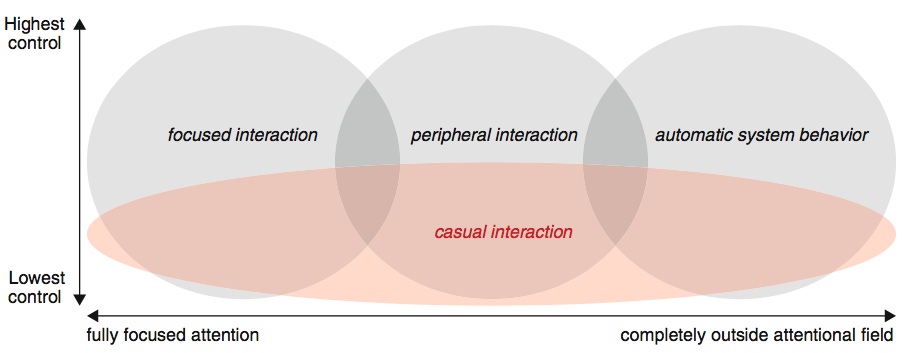
\includegraphics[resolution=300,width=\textwidth]{LevelsOfInteraction}
	\caption{ny.}
	\label{fig:LevelsOfInteraction}
\end{figure}
\noindent
%
\section{Relateret produkter og studier}
\label{RelateretProdukterOgStudier}

I det følgende afsnit er der kigget på hvilke relaterede produkter der findes, samt hvordan perifer interaktion tidligere er blevet studeret og brugt til at styre musik eller lignende.

Tages der udgangspunkt i konceptet omkring et interaktivt kunstværk til væggen findes der flere elektroniske billedrammer på markedet. Nogle af disse billedrammer kan endda styres med gestikker, herilandt Merual \parencite{WEB:Meural} og Framed 2.0 \parencite{WEB:Framed2.0}. Begge disse er billedrammer er en platform, hvor brugeren selv kan vælge, hvad der skal ske på displayet. Den viste kunst kan findes i en database, hvor kunstnere kan uploade og sælge kunst. Brugeren kan på den måde selv vælge hvilket maleri eller andet kunstværk skal vises i billedrammen. Interaktionen med billedrammerne kan ske ved hjælp af en tilknyttet applikation, men begge billedrammer har også bevægelsesensorer knyttet til, så brugeren på den måde kan skifte billedet på skærmen til det næste eller forrige ved hjælp af gestikker. Interaktion ved hjælp af gestikker forudsætter dog, at brugeren er tæt på billedrammen for at sensorene kan opfange bevægelsen. Vendes fokus mod B$\&$O's ønske om at kunne styre et interaktivt kunstværk fra en større afstand, kan der ikke drages mange paralleller mellem det, Merual og Framed 2.0. Dog kan det ud fra billedrammerne forstås, at brugerne er i stand til at interagere med billedrammerne kun ved brug af frihåndsgestikker, hvilket kan medtages til interaktionen med B$\&$O's interaktive kunstværk.

 Udover produkter, der minder om B$\&$O's interaktive kunstværk findes der studier, der har kigget på perifer interaktion til styring af musik og lys. \textcite{PDF:ComparingInputModalitiesForPeripheralInteraction} har undersøgt, hvordan styring af musik, mens brugeren sidder ved en computer, kan finde sted i den perifere del af opmærksomheden. Her blev det først undersøgt hvilke bevægelser der skulle bruges til funktionerne play, pause, skift sang frem/tilbage og volumen op/ned ved henholdsvis brugen af en gribelig knop, en touchflade og fri hånd \parencite[ss. 165-166]{PDF:ComparingInputModalitiesForPeripheralInteraction}. Herefter kørtes et in-situ eksperiment, hvor forsøgspersonerne over otte uger skulle bruge hver af de tre redskaber samt tastaturets egne lydjusteringsknapper til at skifte musikken, mens de brugte deres computer. Ifølge \textcite[ss. 172-173]{PDF:ComparingInputModalitiesForPeripheralInteraction} var styring af musik uden at kigge på musikafspilleren nemmest ved brug af knoppen og touchfladen. Derimod kiggede forsøgspersonerne mere på musikafspilleren ved brug af frihåndsgestikker, da de dels manglede haptisk feedback og dels udtalte at frihåndsgestikkerne føltes magiske, hvilket gjorde at de nød at kigge på musikafspilleren mens de udførte gestikkerne. Ved brug af tasteturets egne lydjusteringsknapper kiggede forsøgspersonerne ifølge data ikke på musikafspilleren, men sagde efter forsøget at de havde kigget på musikafspilleren ved brug af disse. Selvom forsøgspersonerne finder det nemmest at interagere perifert ved brug af knoppen og touchfladen konkluderer \textcite[s. 177]{PDF:ComparingInputModalitiesForPeripheralInteraction} at frihåndsgestikker også egner sig godt til perifer interaktion, i situationer hvor dette er mest passende.
 
  
 
 


%
\begin{itemize}
  \item Meural \parencite{WEB:Meural}
  \item Framed 2.0 
  \item Musikkontrol (kilde med 3 forskellige måder at styre det perifer)
  \item kilde om perifer styring af lysintentises/lysstyrke
\end{itemize}

\chapter{Gestik}
\label{Gestik}
%
I følgende kapitel vil forskellige problemstillinger vedrørende gestik belyses, heriblandt komplikationer forårsaget af gestik, hvilken form for feedback der er nødvendig samt den sociale accept af gestik. Inden da vil der først og fremmest blive undersøgt hvilke former for gestikker, der kan gøres brug af.  
%

\section{Udførelsen af gestik}
\label{UdfoerelseAfGestik}
%
I dette afsnit fokuseres der på to overordnet former for input-gestikker, som et elektronisk apparat kan reagere på. Dernæst fokuseres der på fordelene og ulemperne ved bevægelsesmængden i gestikker. \textcite[s. 9]{PDF:ATaxonomyOfGestures} definerer fem kategorier af gestikker; deiktiske, manipulerende, semaforsike, gestikulerende samt tegnsprog, som uddybes nærmere i \autoref{app:KategoriseringerAfGestikker}. \blankline
%
\textcite[s. 9]{PDF:ATaxonomyOfGestures} definerer to former for inputs et elektronisk apparat kan modtage. Det ene input forekommer enten ved fysisk kontakt med et elektronisk apparat eller et andet objekt, \parencite[s. 10]{PDF:ATaxonomyOfGestures}. Denne form for input henvender sig til at interaktionen foregår via manipulerende gestikker, som defineres i \autoref{app:KategoriseringerAfGestikker}. Ifølge \textcite[s. 12]{PDF:ATaxonomyOfGestures}, er den anden form for input, som et elektronisk apparat kan modtage, baseret på gestikker, som apparatet kan genkende og reagere på ved hjælp af lys-, lyd- eller bevægelsessensorer. Ved denne type input er det derfor muligt at undgå interaktion med eller lokalisering af endnu et elektronisk apparat eller iklæde sig en form for elektronik, som eksempelvis en elektronisk handske, \parencite[s. 12]{PDF:ATaxonomyOfGestures}. Sidst nævnte inputform henvender sig til at interaktionen foregår via semaforiske gestikker, som defineres i \autoref{app:KategoriseringerAfGestikker}. \blankline
%
Bevægelsesmængde indenfor gestik defineres ud fra mikro- og makrogestikker, \parencite[s. 6]{PDF:UsabilityofMicroVsMacroGestures}. Mikrogestikker er små bevægelser, der ikke nødvendigvis kræver, at hele hånden bevæger sig og da de kan udføres samtidig med andre manuelle opgaver, er de specielt lovende indenfor perifer interaktion, \parencite[s. 95]{PDF:PIMicrogesturesKap5}. Ifølge \textcite[s. 96]{PDF:PIMicrogesturesKap5} egner mikrogratikker sig ydermere til perifer interaktion, da de kan udføres hurtigt. Eksempelvis tillader mikrogestikker kommunikation, som en sekundær opgave, samtidig med at fokus holdes på en samtale, som er den primære opgave, uden at samtalepartneren finder én uhøflig, \parencite[s. 97]{PDF:PIMicrogesturesKap5}.

Makrogestikker er derimod store bevægelser, der kræver signifikant bevægelse, som eksempelvis at løfte en arm eller rejse sig fra en siddende position, \parencite[s. 6]{PDF:UsabilityofMicroVsMacroGestures}. Ifølge \textcite[s. 9]{PDF:UsabilityofMicroVsMacroGestures} kan makrogestikker udføres meget mindre præcist end mikrogestikker, da en løftet arm vil tolkes som en løftet arm, uanset om den er løftet 60$^{\circ}$ eller 90$^{\circ}$. En af ulemperne ved makrogestikker er at de kræver et stort areal og at en sensor, som opfanger makrogestikker, ofte vil dække et helt lokale, \parencite[s. 9]{PDF:UsabilityofMicroVsMacroGestures}. Der kan derfor opstå et problem, hvis en anden træder ind i interaktionsområdet og ved et uheld gengiver en bevægelse, som genkendes af systemet. Da det kan være svært at træde ud af interaktionsområdet, kræver det, at brugeren rent fysisk flytter sig langt nok væk, så en ubevidst interaktion undgåes. Til gengæld er en af fordelene ved makrogestikker, at de specifikke gestikker er så tilpas forskellige, at sandsynligheden for at systemet forveksler dem er lille, \parencite[s. 9]{PDF:UsabilityofMicroVsMacroGestures}.  

Mikrogestikker behøver, modsat makrogestikker, ikke et stort interaktionsområde, men skal til gengæld udføres mere præcist, \parencite[s. 10]{PDF:UsabilityofMicroVsMacroGestures}. En af fordelene ved mikrogestikker er, at de tillader en større diversitet end makrogestikker, hvilket gør det muligt at designe flere mikrogestikker end makrogestikker, \parencite[s. 10]{PDF:UsabilityofMicroVsMacroGestures}. En anden fordel ved mikrogestikker er, at interaktionen med systemet sjældent opstår ved en fejl, da det er mindre sandsynligt, at specifikke gestikker udføres ubevidst, \parencite[s. 10]{PDF:UsabilityofMicroVsMacroGestures}. Ulemperne ved mikrogestikker er dels, at desto større afstanden til systemet er, desto større er usikkerheden for, hvorvidt systemet kan registrerer gestikkerne, \parencite[s. 10]{PDF:UsabilityofMicroVsMacroGestures}. Ydermere skal der kompenseres for situationer, hvor brugere skygger for hele eller dele af gestikken, så systemet ikke længere er i stand til at registre og genkende den specifikke gestik. En anden ulempe ved mikrogestikker er brugerens evne til at gengive dem korrekt og uden at forveksle dem. Ifølge \textcite[s. 10]{PDF:UsabilityofMicroVsMacroGestures} egner mikrogestikker sig bedst til situationer, hvor der foretrækkes et mere professionelt udtryk, eksempelvis på arbejdspladsen. Derudover egner mikrogestikker sig også til underholdnings apparater.\blankline
%
I undersøgelsen foretaget af \textcite[s. 823]{PDF:UnderstandingNaturalness} fremgår det, at det er uhensigtmæssigt at benytte sine egne kropsdele til at simulere værktøjer i gestikker, da det føles unaturligt. Med værktøjer refereres der til det værktøj, som ellers vil blive anvendt såfremt det havde været en virkelig situation. Baseret på resultaterne, fremsat i \textcite[s. 823]{PDF:UnderstandingNaturalness}, fremgår det at 77.5 \% af gangene opstår der fejl, når testpersonerne skal anvende en kropsdel som værktøj.

Derimod anbefaler \textcite[s. 823]{PDF:UnderstandingNaturalness}, at gestikkerne udføres som pantomimer, hvor brugere udfører den tiltænkte aktivitet og forestiller sig, at have værktøjet i hånden. Derudover anbefaler \textcite[s. 824]{PDF:UnderstandingNaturalness}, at hvis gestikkerne skal udføres i rummet, altså væk fra det elektroniske apparat, bør gestikkerne udføres med begge hænder. Hvor den ikke-dominante hånd danner en form for ramme eller reference for den dominante hånd, som udfører gestikken.      
%

\section{Komplikationer forårsaget af gestikker}
\label{KomplikationerGestikker}
%
Selvom gestik egner sig til perifer interaktion, er det stadig en forholdvis ny måde at interagere med elektroniske apparater på, \parencite[s. 163]{PDF:ComparingInputModalities}, hvorfor der naturligvis forekommer komplikationer. I følgende afsnit vil nogle af disse komplikationer belyses, først i forhold til teknologiske komplikationer og derefter i forhold til komplikationer vedrørende det menneskeligeaspekt. Fokus vil primært være på sidstnævnte.
%
\subsection{Teknologiske komplikationer}
\label{TeknologiskeKomplikationer}
%
Nogle af de mest åbenlyse teknologiske komplikationer, der kan opstå relaterer sig til problemer med at genkende specifikke gestikker, \parencite[s. 27]{PDF:ATaxonomyOfGestures}. Det gør sig både gældende for mikrogestikker, som er svære at registrere på lang afstand og for makrogestikker, hvor der er risiko for at en anden træder ind i det interaktiveområde og skygger for eller ubevidst udfører gestikker, som genkendes af systemet, \parencite[s. 9]{PDF:UsabilityofMicroVsMacroGestures}. \textit{LeapMotion} udbedrer den teknologiske begrænsning, der forekommer ved mikrogestikker, så snart gestikken udføres tæt på det elektroniske apparat. \textit{LeapMotion} er en lille enhed, som egner sig til at registrere og genkende semaforiske gestikker ved en kort afstand, \parencite[s. 7]{PDF:UsabilityofMicroVsMacroGestures}. Til forskel fra \textit{LeapMotion} anvendes \textit{Microsoft Kinect} til makrogestikker, da dette system er i stand til at genkende helkropsbevægelser, \parencite[s. 4]{PDF:UsabilityofMicroVsMacroGestures}, hvor \textit{LeapMotion} primært relaterer sig til mindre bevægelser, eksempelvis med fingrene. Dog er \textit{Microsoft Kinect} ikke lige så nøjagtigt som \textit{LeapMotion}, hvilket potentielt kan forårsage fejlgenkendelser, hvis to semaforiske gestikker minder om hinanden, \parencite[s. 3]{PDF:UsabilityofMicroVsMacroGestures}. \blankline
%
Særligt ved brug af semaforiske gestikker kan der opstå komplikationer, hvis en naturlig bevægelse fejlagtigt bliver genkendt af et system. Dette velkendte, problem defineres som \textit{Midas touch problem}, der for brugeren kan skabe forvirring, frustration og mistillid til det elektroniske apparat, \parencite[s. 109]{PDF:PIMicrogesturesKap5}. Ydermere kan systemet have problemer med at registrere og genkende semaforiske gestikker, hvis de udføres samtidig med andre bevægelser, \parencite[s. 27]{PDF:ATaxonomyOfGestures}. 

Problemet med semaforiske gestikker opstår, fordi systemet kan have svært ved at registrere både hvornår interaktionen starter og slutter og hvornår det er en sekvens af gestikker fremfor en enkelt gestik, \parencite[s. 27]{PDF:ATaxonomyOfGestures}. For at udbrede dette problem bør brugerne, ifølge \textcite[s. 1]{PDF:DoThatThere}, først og fremmest henvende sig direkte til det pågældende apparat. Det kan potentielt reducere sandsynligheden for at et \textit{Midas touch problem} opstår. I tillæg til at systemet ikke er i stand til at registrere og genkende bestemte gestikker er der, ifølge \textcite[s. 37]{PDF:ATaxonomyOfGestures}, meget få undersøgelser, som fokuserer på brugerens tolerance for at et system begår fejl. Det kan være i forhold til at systemet ikke reagerer på brugerens input, men det kan også være i forhold til at systemet fejlfortolker et input eller registrerer et input, fordi brugeren ubevist udfører en bestemt gestik. \blankline
%
I takt med at teknologi er i konstant udvikling og at virksomheder i elektronikindustrien konstant skal fornye sig og finde nye revolutionerende interaktionformer, antages det, at der er andre virksomheder, som ligeledes undersøger interaktion via semaforiske gestikker. Det forventes derfor at der udvikles flere produkter, hvis interaktion foregår via semaforiske gestikker. Når det er aktuelt, vil der sandsynligvis opstå et problem, som tilnærmelsesvis minder om \textit{Midas touch problem}, hvor det ikke nødvendigvis er brugerens bevægelse, der fejlfortolkes af systemet, men systemerne der fejlfortolker, hvorvidt gestikken er rettet mod dem. For at forbygge og helt undgå et potentielt stort problem foreslår \textcite[s. 2]{PDF:DoThatThere}, at et hvert system først skal addresseres med hver deres unikke gestik, hvorefter brugeren kan interagere med det specifikke system. \blankline
\newpage
%        
En anden teknologisk komplikation kan opstå i designfasen, hvor systemet testes via en \textit{Lo-Fi}-prototype, da der skal tages højde for, at resultaterne fra en \textit{Lo-Fi}-prototype formentligt afviger fra resultaterne fundet i en feltundersøgelse. \textcite[s. 176]{PDF:ComparingInputModalities} oplevede denne afvigelse, hvor testpersonerne fortrak de semaforiske gestikker fremfor de to typer af manipulerende gestikker i testen med \textit{Lo-Fi}-prototypen, hvor det i feltundersøgelsen var de to typer af manipulerende gestikker, som testpersonerne fortrak. Årsagen til det skyldes, ifølge \textcite[s. 176]{PDF:ComparingInputModalities} tre ting; 1) tekniske problemer i forbindelse med semaforiske gestikker i feltundersøgelsen, 2) haptiske problemer og 3) manglende interaktivitet ved \textit{Lo-Fi}-prototypen. 

Derudover er det sjældent at en \textit{Lo-Fi} prototype indeholder den endelige og fuldt funktionelle teknologi, hvorfor testpersonerne, i nogle situationer, nærmere evaluerer konceptet fremfor det endelige produkt. Tages der ikke højde for det i udviklingsfasen, er der risiko for at endelige produkt enten ikke lever op til brugerens ønske eller er for kompliceret at interagere med. Ydermere er det ikke sikkert, at testpersonerne oplever de samme problemer ved en \textit{Lo-Fi}-prototype, som de vil gøre ved det færdige produkt.   
%
\subsection{Komplikationer vedrørende det menneskelige aspekt}
\label{KomplikationerVedroerendeDetMenneskelige}
%
Komplikationer vedrørende det menneskelige aspekt kan opstå ved noget så åbenlyst, som manglende evne til at udføre den specifikke gestik. I den forbindelse kan der opstå problemer ved udmattelse, hvis det er fysisk udmattende at udføre gestikken eller hvis gestikken udføres gentagende gange, \parencite[s. 28]{PDF:ATaxonomyOfGestures}. Derudover indeholder gestikker ikke visuelle hints, hvilket, ifølge \textcite[s. 6]{PDF:NaturalUserInterfaces}, kan være problematisk, hvis systemet ikke reagerer på brugerens bevægelser, eller hvis systemet reagerer forkert. Det skyldes, at brugeren ikke har mulighed for at evaluere den information systemet har registreret og efterfølgende finde ud af, hvad fejlen er. De visuelle hints referer til selve udførelsen af gestikken, hvilket medfører, at når brugeren har udført en bestemt gestik, er det ikke muligt at gense bevægelsen. En måde at undgå denne komplikation på er ved at sørge for, at brugeren modtager en form for feedback, så de dels kan lære af deres fejl og dels ved, hvordan de skal gebærde sig, \parencite[s. 10]{PDF:NaturalUserInterfaces}. I forhold til hvilken type feedback og om der overhovedet skal være feedback vil blive belyst i \fullref{Feedbackformer}. \blankline
%
En anden komplikation, der skal tages højde for, særligt når gestikker anvendes som interaktionsform til perifer interaktion, er, at gestikkerne ikke er perifere før de er lært, inkorporeret og husket, \parencite[s. 16]{PDF:PIEmbeddingHCIOnTheRelevance}. Derudover kræver det, ifølge \textcite[s. 16]{PDF:PIEmbeddingHCIOnTheRelevance}, at opmærksomheden ikke fjernes fra den primære opgave, når der skal interageres i den perifere opmærksomhed, hvilket kun kan opnås, hvis gestikkerne er naturlige. I det henseende pointerer både \textcite[s. 8]{PDF:NaturalUserInterfaces}, \textcite[s. 26]{PDF:ATaxonomyOfGestures} og \textcite[s. 19]{PDF:PIEmbeddingHCIOnTheRelevance}, at der på nuværende tidspunkt både mangler simple og intuitive sets af gestikker og en form for standardisering af gestikker. Såfremt dette efterkommes vil det resultere i, at de samme gestikker repræsenterer og aktiverer de samme funktioner på tværs af de elektroniske apparater. Hvis standardiseringen realiseres, bliver der i den grad brug for, at systemerne kan differentiere mellem, hvornår brugeren henvender sig specifikt til dem og hvornår det ikke er tilfældet, eksempelvis ved at tildele hvert system sin egen unikke aktiveringsgestik, jævnfør \fullref{TeknologiskeKomplikationer}. En af årsagerne til, at der på nuværende tidspunkt ikke forefindes en form for standard og fælles forståelse for hvilke gestikker, der tilhører hvad, skyldes formentlig både, at det er relativt nyt at anvende gestik til interaktion med allestedsværende elektroniske apparater og at det er nyt at anvende gestik i forbindelse med perifer interaktion. Ifølge \textcite[s. 28]{PDF:ATaxonomyOfGestures}, er det usikkert hvilke gestikker, særligt semaforiske gestikker, der passer til bestemte scenarier. Selvom markedet har ændret sig i takt med, at nye teknologier finder indpas og selvom vores måde at interagere med disse teknologier ligeledes har ændret sig i forhold til, hvordan det var i 2005, før smartphones florerede på markedet, er det yderst relevant at undersøge hvilke semaforiske gestikker, der egner sig bedst til specifikke scenarier, hvor interaktionen foregår i den perifere opmærksomhed.

En gennemgående diskussion vedrørende semaforiske gestikker er at de betragtes som værende unaturlige, \parencite[s. 1961]{PDF:AStudyOnTheUseOfSemaphoricGestures}, men samtidig er det den form for gestik, der er mest udbredt indenfor interaktion med allestedsværende elektroniske apparater, \parencite[s. 28]{PDF:ATaxonomyOfGestures}. Ydermere understøtter semaforiske gestikker interaktion, der ikke afhænger af den visuelle opmærksomhed, \parencite[s. 1964]{PDF:AStudyOnTheUseOfSemaphoricGestures}, hvilket er favorabelt i forbindelse med perifer interaktion. Der kan være en fordel i at semaforiske gestikke ikke nødvendigvis er fuldstændig naturlige, da helt naturlige gestikker kan skabe problemer, \parencite[s. 9]{PDF:NaturalUserInterfaces}. \textcite[s. 9]{PDF:NaturalUserInterfaces} belyser problemet med naturlige gestikker i forbindelse med bowling spillet til Nintendo Wii, som forårsagede ødelagte fjernsyn. Spillet skal gengive et almindeligt spil bowling, hvor kontrollen svinges ligesom bowlingkuglen. Når spilleren normalvis slipper bowlingkuglen, kom spilleren naturligt til at slippe Nintendo Wii kontrollen, som derefter røg direkte ind i fjernsynet og ødelagde skærmen. Det bør derfor genovervejes hvor naturlige gestikkerne ønskes, da det kan være en fordel at gøre dem mindre naturlige, som tilfældet ved semaforiske gestikker.
%

\section{Feedbackformer}
\label{Feedbackformer}
%
Der er en del udbredte meninger om, hvorvidt der skal være feedback i alle interaktionssituationer samt hvilken type feedback, der skal anvendes. Diskussionen omkring feedbackformer vil primært omhandle semaforiske og manipulerende gestikker i forbindelse med at interagere med et musikanlæg, hvilket er oplagt fordi projektet er et samarbejde med Bang $\&$ Olufsen, \fullref{SamspilMedBO}. \blankline
%
\textcite[s. 10]{PDF:NaturalUserInterfaces} argumenterer for, at der skal være feedback, for på den måde at hjælpe brugeren til at forstå årsagen til eventuelle fejl og dertil lære den korrekte adfærd. Hvorimod \textcite[s. 16]{PDF:PIEmbeddingHCIOnTheRelevance} argumenterer for, at hvis gestikkerne er semaforiske, så er det ikke nødvendigt med, hvad \textcite[s. 16]{PDF:PIEmbeddingHCIOnTheRelevance} kategorisere som værende augmenteret feedback, da brugeren automatisk får feedback fra den proprioceptive sans, når der sker en aktivering af musklerne. På baggrund af det argumenterer \textcite[s. 16]{PDF:PIEmbeddingHCIOnTheRelevance} ydermere for, at det er derfor, at semaforiske gestikker egner sig til perifer interaktion. I henhold til semaforiske gestikker, så gav testpersonerne, i undersøgelsen foretaget af \textcite[ss. 172-173]{PDF:ComparingInputModalities}, udtryk for, at de manglede haptisk feedback. Årsagen til det skyldes formegentligt, at testpersonerne først og fremmest skal vænne sig til og stole på de semaforiske gestikker, hvorefter der formegentlig ikke længere er behov for haptisk feedback, \parencite[s. 174]{PDF:ComparingInputModalities}. 

Derudover argumenterer \textcite[s. 3]{PDF:FacilitatingPIDesignAndEvaluation} for, at det er problematisk at give brugeren feedback igennem den samme sensoriske modalitet, hvor opgaven befinder sig, da der kan opstå interferens. Derfor er det uhensigtmæssigt og mindre brugbart at anvende auditiv feedback, når brugeren samtidig lytter til musik, \parencite[s. 3]{PDF:FacilitatingPIDesignAndEvaluation}. I tilfælde hvor brugeren perifert skal interagere med et musikanlæg, kommenterer \textcite[s. 19]{PDF:PIEmbeddingHCIOnTheRelevance}, at brugeren i forvejen modtager feedback i form af funktionel feedback, hvor brugeren kan høre at musikken pauses, at der justeres på lydstyrken eller at der skiftes musiknummer. \textcite[s. 3]{PDF:InteractionFrogger} definerer funktionel feedback, som værende den information, som generes når en funktion initieres, svarende til at hvis brugeren gengiver gestikken, som pauser musikken så vil den funktionelle feedback være, at musikken stopper med at spille. 

Hvis perifere interaktion foregår igennem manipulerende gestikker, så har ikke-visuel feedback potentiale for at minimere belastningen af de mentale ressourcer, \parencite[s. 3]{PDF:FacilitatingPIDesignAndEvaluation}. Dog giver testpersonerne, i undersøgelsen foretaget af \textcite[s. 173]{PDF:ComparingInputModalities}, udtryk for, at de ikke manglede yderligere feedback end det de fik fra den funktionelle feedback. Hvor den funktionelle feedback i dette tilfælde vedrører den proprioceptive sans, fordi testpersonerne manipulerer et fysisk objekt, et knop-baseret håndtag og touchskærmen, og de kan høre at systemet reagerer på inputtet.

Udover funktionel feedback definerer \textcite[s. 3]{PDF:InteractionFrogger}, yderligere to feedbackformer; augmenteret og iboende feedback, hvor førstnævnte gengiver at feedbacken kommer fra en ekstern kilde, modsat iboende feedback, som gengiver at feedbacken kommer direkte fra, hvor interaktionen foregår. \blankline
%
\textcite[ss. 1263-1268]{PDF:ComparingModFeedback} undersøger om forskellige feedback typer, fra visuel feedback i den perifere opmærksomhed til feedback direkte på skærmen, har en effekt på testpersonernes præstationsevne. Ifølge \textcite[ss. 1267-1268]{PDF:ComparingModFeedback} har feedback ingen effekt på præstationsevnen i den sekundære opgave, men testpersonerne efterspørger alligevel feedback, så de kan få information omkring deres handlinger. Lignende resultater forefindes i en undersøgelse foretaget af \textcite[s. 8]{PDF:DoThatThere}, som ligeledes ikke finder at feedback har en effekt på præstationsevnen. Dog tyder det på, at feedback er med til at gøre det nemmere for testpersonerne at interagere med gestikker, \parencite[s. 8]{PDF:DoThatThere}. Ligesom \textcite[s. 174]{PDF:ComparingInputModalities} argumenterer \textcite[s. 1268]{PDF:ComparingModFeedback} for, at det ikke nødvendigvis vil være tilfældet i en feltundersøgelse da testpersonerne får længere tid til at vænne sig til den perifere interaktion. 

Det lader derfor til at testpersoner, som testes i et laboratorium, har andre behov, end hvis de blev testet i en feltundersøgelse. Det kan derfor være svært at afgøre, hvorvidt der skal være en form for feedback eller ej, når en bruger interagerer med et musikanlæg i den perifere opmærksomhed. Dette gør sig særligt gældende, når interaktionsformen enten bygger på semaforiske og/eller manipulerende gestikker. \blankline 
%
For at undgå nogle af de komplikationer, der blev adresseret i \fullref{KomplikationerGestikker}, foreslår \textcite{PDF:DoThatThere}, at det ved hjælp af feedback er muligt at inddele interaktionen i to; \textit{Do that} og \textit{There}. Formålet med \textit{Do that} er, at hjælpe brugeren til at udføre de korrekte handlinger, hvortil \textcite[s. 4]{PDF:DoThatThere} undersøger, hvad de definerer som rytmiske gestikker. Rytmiske gestikker vedrører at få brugeren til at udføre bevægelsen i takt med at systemet eksempelvis lyser i et bestemt mønster, som brugeren skal efterligne. Brugeren får dermed bekræftet, at en specifik gestik er registreret og ligeledes undgår brugeren, at systemet reagerer på gestikker, som ikke er henvendt til systemt, \parencite[s. 4]{PDF:DoThatThere}. \textcite[s. 10]{PDF:DoThatThere} anbefaler, at brugeren får feedback fra de rytmiske gestikker fra det tidspunkt interaktionen begynder. Ydermere anbefaler \textcite[s. 10]{PDF:DoThatThere}, at så snart det er muligt så skal de rytmiske gestikker gengives ved enten horisontale eller vertikale bevægelser. 

Formålet med \textit{There} er, ved hjælp af feedback, at vejlede brugeren til, hvor gestikken skal udføres, for at den kan registreres. \textcite[s. 10]{PDF:DoThatThere} anbefaler, at vejlede brugeren til det korrekte sted for at udføre gestikken, ved hjælp af lys. 


\subsection{Er semaforiske gestikker social acceptable?}
\label{Socialaccept}
%            
Grunden til, at der ikke fokuseres på hverken manipulerende eller deiktiske gestikker i forhold til social accept skyldes, at ved begge tilfælde er hele interaktionen og resultatet af interaktion synlig. Det er muligt for tilskuere, at se hvad en gestik medfører, uanset om det er ved at manipulere et objekt eller ved at pege på et objekt. Ydermere antages det at manipulerende gestikker er så veletableret, at både tilskuere og brugeren selv ikke nødvendigvis tænker over, at det er en gestik. \blankline
%
Af de fire undersøgelser, som det har været muligt at finde, fremgår det, at fokus har været på social accept af semaforiske gestikker, \parencite{PDF:AChairAsUbiquitousInputDevice, PDF:WouldYouDoThat, PDF:AreYouComfortableDoingThat, PDF:AnExploratoryStudy}. Af de fire undersøgelser fokuserer \textcite{PDF:AreYouComfortableDoingThat} og \textcite{PDF:WouldYouDoThat} på hvordan semaforiske gestikker opfattes af andre samt i hvilke situationer brugeren er villig til og komfortable ved at udføre bestemte former for semaforiske gestikker og hvornår de ikke er. I undersøgelsen foretaget af \textcite{PDF:AnExploratoryStudy} fokuseres der på, hvordan sociale elektroniske apparater kan være med til at fremme kontakten mellem mennesker. Hvor der i undersøgelsen, foretaget af \textcite{PDF:AChairAsUbiquitousInputDevice}, fokuseres på en interaktiv stol. Interaktionen undersøges i to scenarier; i den centrale opmærksomhed hvor testpersonerne interagere med en computer og i den perifere opmærksomhed hvor testpersonerne interagere med en musikafspiller, \parencite{PDF:AChairAsUbiquitousInputDevice}. Ved begge scenarier giver testpersonerne udtryk for, at de er bekymret for hvorvidt deres interaktion er social acceptabel, \parencite[s. 8]{PDF:AChairAsUbiquitousInputDevice}. Bekymringerne vedrører, hvorvidt andre anser gestikkerne, som værende akavet, \parencite[s. 4]{PDF:AChairAsUbiquitousInputDevice}. Dog pointerer \textcite[s. 9]{PDF:AChairAsUbiquitousInputDevice}, at det kan hænge sammen med, at gestikken er synlig men resultatet deraf er usynligt, det er derfor kun testpersonen, der kan høre at musikken ændre sig. \textcite[s. 9]{PDF:AChairAsUbiquitousInputDevice} argumentere for, at hvis den interaktive stol implementeres i et i forvejen interaktivt miljø, så kan det potentielt reducere den akavede fornemmelse.\blankline
%
Der er overordet to måder at definere social accept; ud fra brugerens syn eller ud fra tilskuerens syn. Ud fra brugerens synspunkt handler social accept om det indtryk brugeren får ved at udføre interaktionen, var oplevelsen positiv eller negativ, \parencite[s. 276]{PDF:WouldYouDoThat}. Hvor social accept ud fra tilskuerens synspunkt afhænger af hvordan tilskueren vurderer brugerens adfærd som værende enten positiv eller negativ, \parencite[s. 276]{PDF:WouldYouDoThat}. Ifølge \textcite[s. 276]{PDF:WouldYouDoThat} påvirker følgende faktorer social accept; brugertype, tid og sted samt manipulation kontra effekt. Brugertype henviser til om brugeren hurtigt accepterer gestik, som interaktionsform eller om de stritter i mod. Tid og sted henviser til kultur og hvor længe den pågældende teknologi har været på markedet, hvilket kan være med til at øge den sociale accept. Manipulation kontra effekt henviser til de specifikke gestikker og hvad de resulterer i, hvilket vil blive uddybet yderligere.

Ifølge \textcite[s. 276]{PDF:WouldYouDoThat} kan gestikker inddeles i følgende fire kategorier; udtryksfyldte, spændingsfyldte, hemmelighedsfyldte og magiske. Hvor de udtryksfyldte gestikker både har synlig manipulation og synlig effekt modsat de hemmelighedsfyldte gestikker, som både har usynlig manipulation og usynlig effekt. De magiske gestikker defineres, som de gestikker hvor manipulationen er usynlig men effekten er synlig, modsat de spændingsfyldte som har synlig manipulation og usynlig effekt. Baseret på resultaterne fremsat af \textcite[s. 277]{PDF:WouldYouDoThat} fremgår det, at de spændingsfyldte gestikker ikke anses for, at være socialt acceptable, det gælder både i offentlige og private sammenhænge. De hemmelighedsfyldte gestikker, derimod blev rangeret højt i forhold til social accept både i det offentlig og i det private. Ydermere fremgår det ligeledes af resultaterne, at både de udtryksfyldte og magiske gestikke generelt opleves, som værende social acceptable, \parencite[s. 277]{PDF:WouldYouDoThat}. 

Det tyder derfor på, at gestikker hvor manipulationen er synlig nødvendigvis også må have en synlig effekt for at blive social accepteret. Alternativt kan manipulationen være usynlig, hvor effekten enten kan være synlig og usynlig, for stadig at opnå social accept, \parencite[s. 278]{PDF:WouldYouDoThat}. Disse kategorier inden for social accept er uafhængige af kategoriseringen i \fullref{KategoriseringerAfGestikker}, i den forstand at de ikke er koblet til én specifik form for gestik men nærmere hænger sammen med hvordan gestikken udføres.\blankline
%
I undersøgelsen foretaget af \textcite[s. 193]{PDF:AreYouComfortableDoingThat}, fokuseres der dels på den sociale accept og dels på om brugeren føler sig komfortabel ved, at udføre gestikker i området omkring et elektronisk apparat. Det fremgår, at der er en stærk forbindelse mellem gestikkens nødvendige bevægelsesmængde, varigheden hvormed gestikken udføres samt positionen, relativt til det elektroniske apparat, \parencite[s. 193]{PDF:AreYouComfortableDoingThat}. Derudover fremgår det ligeledes at brugere er både selektive og bevidste om hvor interaktionen foregår, privat eller offentligt, samt hvem der kan se denne interaktion, \parencite[s. 193]{PDF:AreYouComfortableDoingThat}. Denne problemstilling undersøges i tre forskellige henseende; 1) området og afstanden fra det elektroniske apparat, 2) Bevægelsesmængden og varigheden af gestikken og 3) Tilskuere, \parencite[ss. 195-200]{PDF:AreYouComfortableDoingThat}. 

Ud fra den første undersøgelse fremgår det at testpersonerne føler sig mest komfortable ved at udføre gestikkerne i området tæt på, lige over og helst til højre for det elektroniske apparat, \parencite[s. 197]{PDF:AreYouComfortableDoingThat}. Endvidere vurderer \textcite[s. 201]{PDF:AreYouComfortableDoingThat}, at grænsen for hvornår en gestik er i risiko for, at blive anset som værende social uacceptabel er når afstanden til det elektroniske apparat når 30cm. I forhold til hvem testpersonerne føler sig komfortable ved, når de skal udføre gestikkerne, fremgår det, at det primært er personer, som de har et tæt forhold til, såsom venner, familie og deres partnere, \parencite[s. 196]{PDF:AreYouComfortableDoingThat}. Dertil føler testpersonerne sig mest ukomfortable overfor fremmede og kollegaer, \parencite[s. 196]{PDF:AreYouComfortableDoingThat}. Testpersonerne vurdere, ydermere, at de to mest ukomfortable lokationer, at udføre gestikkerne på er i offentligtransport og på et museum, \parencite[s. 196]{PDF:AreYouComfortableDoingThat}. 

Ved den næste undersøgelse, som vedrører bevægelsesmængde og varighed, defineres en bevægelsesmængde inden for et område på 15x15cm., som værende lille, hvorimod hvis gestikken udføres inden for et område på 30x30cm., så anses bevægelsesmængden for at være stor, \parencite[s. 198]{PDF:AreYouComfortableDoingThat}. Gestikkerne udføres ved tre forskellige varigheder; tre sekunder, seks sekunder og ni sekunder. På baggrund af resultaterne fra undersøgelse 2) fremgår det, at gestikker med en varighed på mindre end seks sekunder klart er at fortrække, hvis testpersonerne skal føle sig komfortable, \parencite[s. 199]{PDF:AreYouComfortableDoingThat}. Ydermere foretrækker testpersonerne en lille bevægelsesmængde, dog pointere \textcite[s. 199]{PDF:AreYouComfortableDoingThat}, at såfremt en gestik med en stor bevægelsesmængde udføres i en favorabel lokation, tæt på det elektroniske apparat, og har en kort varighed så kan der kompenseres for den ellers ukomfortable oplevelse. 

Ved den tredje undersøgelse, som vedrører tilskuerne, fremgår det, at tilskuerne ikke fandt gestikkerne påtrængende og en del af tilskuerne tænkte ikke yderliger over de gestikker, som de lige havde overværet, \parencite[s. 200]{PDF:AreYouComfortableDoingThat}. Ifølge \textcite[s. 200]{PDF:AreYouComfortableDoingThat} så har tilskuerne en tendens til, at vurderer den sociale accept en del højere end hvad tilfældet var ved de to foregående undersøgelser. \blankline
%
\textcite{PDF:AnExploratoryStudy} undersøger, hvordan semaforiske gestikker kan understøtte interaktionen med elektroniske apparater, som fremme den sociale kontakt mellem mennesker. Baseret på disse resultater tyder det på, at gestikker med en stor bevægelsesmængde kan være social acceptable og komfortable, hvis de udføres hjemme hos ens venner, \parencite[s. 4]{PDF:AnExploratoryStudy}. Endvidere finder testpersonerne det mindre pinligt, at udføre gestikker fremfor både stemmestyring og lydkontrol, \parencite[s. 4]{PDF:AnExploratoryStudy}. Ydermere fremgår det, at testpersonerne foretrækker, at gestikkerne benyttes i en positiv sammenhæng fremfor en negativ sammenhæng, hvor de foretrækker at gestikkerne da er mindre synlige, \parencite[s. 4]{PDF:AnExploratoryStudy}. \blankline
%
Så for at svare på om semaforiske gestikker er social acceptable, så afhænger det af flere aspekter, dels hvilket miljø gestikken optræder i, forholdet mellem manipulation og effekt i forhold til hvad der er synligt kontra usynligt, gestikkens bevægelsesmængde og varighed, området og afstanden til det elektroniske apparat og hvilken type tilskuere, der overvære gestikken. For at opsummere nogle af de anbefalinger, der fremgår i de fire undersøgelser, så tyder det på, at i forhold til miljø så er brugerene mere tilbøjelige til at føle sig komfortable i private omgivelser og såfremt gestikken udføres i det offentlige, så skal den være forholdvist diskret. En af årsageren til, at testpersonerne i undersøgelsen, foretaget af \textcite[s. 4]{PDF:AChairAsUbiquitousInputDevice}, gav udtryk for bekymringer i forbindelse med interaktionen med den interaktive stol, kan formegentlig skyldes, at i det tilfælde var manipulationen synlig og effekt var usynlig for tilskuerne, svarende til hvad \textcite[s. 276]{PDF:WouldYouDoThat}, definerer til at være en spændingsfyldt gestik.  

I forbindelse med manipulation og effekt, så anbefaler \textcite[s. 278]{PDF:WouldYouDoThat}, at der netop ikke bruges spændingsfyldte gestikker hvor manipuleringen er synlig og effekten er usynlig, hvilket efterlader de udtryksfyldte, hemmelighedsfyldte og magiske gestikker til fri afbenyttelse for at opnå social accept. I relation til bevægelsesmængden så anbefaler \textcite[s. 201]{PDF:AreYouComfortableDoingThat}, at såfremt gestikken udføres i det offentlige, så skal der være en forholdvist lille bevægelsesmængde i et område svarende til 15x15cm. Ifølge \textcite[s. 278]{PDF:WouldYouDoThat}, så er både små og store bevægelsesmængder socialt acceptable, så længe effekten er synlig.

Ydermere skal varigheden være kortere end seks sekunder, da risikoen for at brugeren da føler sig ukomfortabel stiger. I forbindelse med området og afstanden vurderer \textcite[s. 201]{PDF:AreYouComfortableDoingThat}, at området til højre og foran det elektroniske apparat er at foretrække, særligt for højrehåndet brugere, ellers skal der tages højde for afstanden. Ifølge \textcite[s. 201]{PDF:AreYouComfortableDoingThat}, så er grænsen for, hvornår det er komfortabelt samt social acceptabelt, omkring 30cm mellem det elektroniske apparat og gestikken.\blankline
%
Igennem \fullref{Gestik} er der blevet belyst dels hvilke kategorier forskellige former for gestik tilhører, komplikationer forårsaget af gestikker, feedbackformer og hvorvidt semaforiske gestikker anses for at være social acceptable. Der er i \fullref{KategoriseringerAfGestikker} blevet afgrænset fra, at arbejde videre med tegnsprog og gestikulerende gestikker. I forhold til hvilke komplikationer, der er forårsaget af gestik, er det primære fokus rettet mod det menneskelige aspekt, for på den måde at undersøge hvilke gestikker, der bedst egner sig til perifer interaktion med et musikanlæg eller en musikafspiller. Dertil skal det overvejes hvor meget fokus, der skal rettes mod feedbackformer, da der ikke er en fælles konsensus om hvorvidt der skal være feedback i situationer, hvor der i forvejen fremgår funktionel feedback både i forhold til gestikkerne og i forhold til musikken. Såfremt den perifere interaktion udføres med semaforiske gestikker, så er der nogle faktorer, der skal tages højde for i forbindelse med brugernes og tilskuernes sociale accept.\blankline
% 
På baggrund af de foregående afsnit er det nu muligt, at konkretisere projektets fokus, igennem en afgrænsning, som efterfølgende munder ud i en problemformulering.  









\chapter{Projekt afgrænsing}
\label{Afgraensning}
%
%
Igennem \fullref{Gestik} er der blevet belyst, hvilke kategorier forskellige former for gestik tilhører, komplikationer forårsaget af gestikker, feedbackformer og hvorvidt semaforiske gestikker anses for at være social acceptable. Der er i \fullref{KategoriseringerAfGestikker} blevet afgrænset fra, at arbejde videre med tegnsprog og gestikulerende gestikker. I forhold til hvilke komplikationer, der er forårsaget af gestik, er det primære fokus rettet mod det menneskelige aspekt, for på den måde at undersøge hvilke gestikker, der bedst egner sig til perifer interaktion med et musikanlæg eller en musikafspiller. Dertil skal det overvejes hvor meget fokus, der skal rettes mod feedbackformer, da der ikke er en fælles konsensus om, hvorvidt der skal være feedback i situationer, hvor der i forvejen fremgår funktionel feedback både i forhold til gestikkerne og i forhold til musikken. Såfremt den perifere interaktion udføres med semaforiske gestikker, så er der nogle faktorer, der skal tages højde for i forbindelse med brugernes og tilskuernes sociale accept.\blankline
% 
På baggrund af de foregående afsnit er det nu muligt, at konkretisere projektets fokus, igennem en afgrænsning, som efterfølgende munder ud i en problemformulering.  
%
I følgende afsnit opsummeres og specificeres, hvilken tilgang til perifer interaktion med et musikanlæg, der fremadrettet vil blive fokuseret på i samarbejdet med Bang $\&$ Olufsen. Dertil vil der dels blive afgrænset fra nogle af de føromtalte problemstillinger, som fremgår af de forgående afsnit, og dels præciseres hvilke der arbejdes videre med, til det vil der blive udarbejdet en problemformulering.\blankline
% 
Da der ikke findes én universal måde, at interagere med produkter i den perifere opmærksomhed, så er det fordelagtigt, at interaktionen med et specifikt produkt undersøges nærmere. Der vil derfor kun blive fokuseret på den perifere interaktion med et musikanlæg fra Bang $\&$ Olufsen. På baggrund af \fullref{PeriferInteratkion} fremgår det, at for bedst at understøtte perifer interaktion, er det er en fordel at undgå, at interaktionen skal foregå i den visuelle opmærksomhed. Ved at afgrænse sig fra interaktion i den visuelle opmærksomhed, vil det i højere grad være muligt, at designe en interaktionsform, som ikke længere kræver at brugeren allokere sin centrale opmærksomhed og dermed afbryder sin primære opgave midlertidigt. Derudover så tyder det på, at der til perifer interaktion kan drages stor nytte af den proprioceptive sans, som netop tillader interaktion uafhængigt af den visuelle opmærksomhed, jævnfør \fullref{Potentiale}. Der bliver ydermere afgrænset fra stemmestyring, dels fordi det anses for at være for krævende og derfor ikke kan foregå i det perifere, \parencite[s. 41]{PDF:PIEmbeddingHCIMicroManageMe}, og dels fordi det betragtes, som værende mere pinligt end at udføre gestikker, \parencite[s. 4]{PDF:AnExploratoryStudy}.        

Som belyst i \fullref{KategoriseringerAfGestikker} findes der forskellige kategorier af gestikker, hvoraf nogen egner sig bedre til perifer interaktion end andre. Til interaktion med Bang $\&$ Olufsens fremtidige musikanlæg tyder det på, at semaforiske gestikker vil være gunstige. Det understøttes, blandt andet, af at det er en af de interaktionsformer, som andre har haft stor gavn af, jævnfør \fullref{RelateretUndersoegelser}. Derudover understøtter semaforiske gestikker den proprioceptive sans, da de ikke kræver, at brugeren skal være i besidelse af endnu en form for fjernbetjening og det er muligt at interaktionen kan foregå i den perifere opmærksomhed. Ydermere blev det uddybet, at gestikker kan kategoriseres efter bevægelsemængde i henholdsvis mikro- og makrogestikker. Da det forventes, at interaktionen med musikanlægget kan foregå ved forskellige afstande og op mod fire meter til brugeren, er det ikke på nuværende tidspunkt muligt at afgrænse sig til udelukkende at arbejde med enten mikro- eller makrogestikker. Der kan dog være en fordel i, særligt i forhold til social accept og hvorvidt brugeren føler sig komfortabel med at udføre de semaforiske gestikker, at designe de semaforiske gestikker så de kan foregå tæt på brugerens egen krop. Det tilstræbes derfor, at komme frem til en form for kompromis mellem decideret mikro- og makrogestikker, da de hver især bidrager med dels noget positivt og dels med noget negativt, jævnfør \fullref{UdfoerelseAfGestik}.\blankline
%
I \fullref{KomplikationerGestikker} præsenteres nogle af de komplikationer, som gestikker kan forårsage, det gælder både teknologiske såvel som menneskelige komplikationer. Der afgrænses i dette projekt fra, at undersøge det tekniske aspekt nærmere, da formålet med projektet primært retter sig mod, at finde en måde hvorpå brugerene kan interagere med Bang $\&$ Olufsens fremtidige musikanlæg perifert. Da Bang $\&$ Olufsens fremtidige musikanlæg på nuværende tidspunkt befinder sig på konceptbasis, er det ikke muligt at foretage feltundersøgelser ej heller udføre Hi-Fi tests, dog vil det blive forsøgt, at tilstræbe et så naturligt testscenarie, som muligt. Selvom der afgrænses fra det teknologiske aspekt tilstræbes det dog, at de semaforiske gestikker ikke designes til stor hinder for teknologien. Det forventes derfor ikke at teknologien kan registre semaforiske gestikker, som enten er delvist eller fuldstændig dækket af andre objekter.  

At anvende semaforiske gestikker, som interaktionsform i den perifere opmærksomhed er stadig forholdvist nyt, så der findes endnu ikke et standard sæt af gestikker, som henvender sig til musikkontrol, i hvert fald ikke hvad der er projektgruppen kendt. Det vil derfor være nødvendigt, at foretage en dybere undersøgelse af netop hvilke semaforiske gestikker, der egner sig bedst til nogen af de mest gængse funktioner et musikanlæg indeholder; start, pause, justering af lydstyrken og skift musiknummer frem og tilbage. Ydermere er det interessant at undersøge, om der findes semaforiske gestikker, der trods deres unaturlighed kan læres og genkaldes og på den måde benyttes til perifer interaktion. Der skal dog tages højde for, at disse gestikker ikke skal afspejle almindelige, naturlige gestikulerende gestikker, der eksempelvis opstår ved samtale, da risikoen for at udføre en gestik ved en fejl vil stige. Det findes derfor interessant at undersøge lige netop det område, hvor semaforiske gestikker fejlfrit kan benyttes til HCI i den perifere opmærksomhed. \blankline
%
Undersøges behovet for feedback ved perifer interaktion, er der, som beskrevet i \fullref{Feedbackformer}, delte meninger. Der bliver både argumenteret for, at det ikke er nødvendigt med augmenteret feedback ved semaforiske gestikker, grundet den funktionelle feedback fra den proprioceptive sans og fordi brugeren ydermere får funktionel feedback i og med at musikken ændre sig afhængigt af inputtet. Der bliver også argumenteret for at den funktionelle feedback ikke er nok, for selvom feedback ikke nødvendigvis fremmer brugerens præstationsevne, så er feedbacken med til, at hjælpe dem igennem interaktionen. Fokus for dette projekt vil i første omgang ikke være rettet direkte mod at designe en bestemt form for feedback, men feedback vil undervejs blive holdt in mente, såfremt det skulle blive relevant. Det skyldes, blandt andet, at \textcite[s. 21]{PDF:FacilitatingPIDesignAndEvaluation} hævder at multimodal feedback, som er feedback der registreres af flere sanser, styrker perifer interaktion. Da der ikke afgrænses fuldstændigt fra at arbejde med feedback og det samtidig er et betydningsfyldt aspekt inden for interaktions design, så vil feedback blive yderligere diskuteret fremadrettet.  

Det er ikke muligt at forudbestemme præcist, hvordan gestikkerne skal udføres, da der skal tages højde for dels, om brugeren føler sig komfortable ved at udføre dem og dels, om mulige tilskuer oplever denne nye form for interaktion, jævnfør \fullref{Socialaccept}. På nuværende tidspunkt kan der med sikkerhed afgrænses fra at bruge spændingsfyldte gestikker, da disse ikke anses for at være socialt acceptable, \parencite[s. 277]{PDF:WouldYouDoThat} og hemmelighedsfyldte gestikker, da det ikke vil give meget mening ved interaktion med et musikanlæg, fordi det vil være svært og uhensigtmæssigt at skjule effekten af en gestik. Tilbage er der de udtryksfyldte- og magiske gestikker, som begge egner sig til interaktion med et musikanlæg og til perifer interaktion. Derudover lægger Bang $\&$ Olufsen vægt på, at brugeroplevelsen føles magisk, så det vil give mening, at undersøge om de magiske gestikker, som er defineret af \textcite[s. 276]{PDF:WouldYouDoThat} til at være gestikker hvor manipulationen er skjult og effekten er synlig, egner sig til at fremme denne brugeroplevelse. \blankline
%
Projektet er nu afgrænset til at undersøge, hvordan perifer interaktion kan foregå med semaforiske gestikker, når et musikanlæg skal styres fra en vilkårlig afstand, hvilket danner grundlag for en problemformulering.

\section{Problemformulering}
\label{Problemformulering}

Ved samarbejde med Bang $\&$ Olufensen er det altså et ønske at undersøge, hvordan der kan interageres med et interaktivt kunstværk, uden at det skal forstyrre primære opgaver som eksempelvis samtale. Måden, hvorpå der skal interageres, er ved brug af semaforiske gestikker, der signalerer hvordan musikken skal ændre sig uden at dette skal forstyrre, fejltolkes eller fremstå socialt uaccetabelt. For at få interaktionen med produktet til at fremstå gnidningsløst og magisk opstilles følgende problemstillinger, som der i projektet vil blive forsøgt svaret på.\\

\begin{itemize}
	\item Hvilke af de primære funktioner kan udføres med semaforiske gestikker?
	\item Hvilke semaforiske gestikker kan bruges til de primære funktioner, som det giver mening at have tiknyttet gestikker?
	\item Kan de semaforiske gestikker bruges til perifer interaktion uden at gestikkerne bliver lavet ubevidst?
	\item Er de semaforiske gestikker socialt acceptable?\\
\end{itemize}
For at besvare de forskellige problemstillinger kan flere brugerundersøgelser udføres, herunder kliniske undersøgelser, hvor brugerens holdning til forskellig gestikker kommer til udtryk, og mere virkelighedsnære undersøgelser, hvor gestikkerne bliver testet i en brugssituation.

\newcommand{\ValgAfGestikkerpartname}{Valg af gestikker}
\newcommand{\ValgAfGestikkerparttext}{Ny 
\newpage 
}
%
\part[\ValgAfGestikkerpartname]{\ValgAfGestikkerpartname
\label{\ValgAfGestikkerpartname}
\vspace{8mm}
	\begin{center}
		\begin{minipage}[l]{14cm}
			\textnormal{\normalsize\noindent\ValgAfGestikkerparttext}
		\end{minipage}
	\end{center}
}


\chapter{Analyse af semforiske gestikker}
\label{AnalyseAfSemaforiskeGestikker}
%

\begin{itemize}
  \item Indledning til afsnittet
  \item opsummering af hvilke gestikker vi ikke vil og gerne vil kigge på.
  \item Forklaring af de forskellige gestikker der kan bruges
  \begin{itemize}
  	\item Gestikker fra litteraturen
  	\item Gestikker overført fra Bang $\&$ Olufsens eksisterende produkter
  	\item Vores egne idéer til gestikker
  \end{itemize}
  \item Fordele og ulemper ved gestikkerne
  \item Hvordan brugerundersøgelsen opstilles og udføres
  \item Resultater fra brugerundersøgelsen
  \item konklusion på brugerundersøgelsen og videre arbejde
\end{itemize}


 



\chapter{Diskussion}
\label{Samlet Diskussion}
%
\begin{itemize}
  \item Har i et bud på hvorfor der er et gab, mellem fokuseret og automatisk interaktion (perifer) Lars Bos kommentar!
  \item Gamle telefoner med knapper var perifert
\end{itemize}

\chapter{Konklusion}
\label{Konklusion}
\chapter{Perspektivering}
\label{Perspektivering}
Hvilken cool gesture kan vi lave, hvis man vil shuffle musikken?

In-situ test, når prototypen er færdig

%%%% Kilder %%%%
\printbibliography	%Litteraturlisten inkluderes

%%%% Bilag %%%%
\appendix
\appendixpage
%Skriv kort introduktion til hvert bilag

% For .TEX:
%\input{FILSTI/FILNAVN}

% For .PDF:
%\chapter{NAVN}
%\label{app:LABEL}
%\includepdf[pages={-}]{FILSTI/FILNAVN}
%\chapter{ISO226 Data}
\label{app:ISO226Raadata}
%
Lydtryksniveauer til de otte phon-kurver i det opgivne frekvensområde, svarende til hvad der er opgivet i \textcite[ss. 6-7]{STD:ISO226}.
%
\begin{table}[H]
\centering
\resizebox{\textwidth}{!}{%
\begin{tabular}{|r|r|r|r|r|r|r|r|r|}
\hline
Frekvens{[}Hz{]} & \multicolumn{1}{l|}{20phon} & \multicolumn{1}{l|}{30phon} & \multicolumn{1}{l|}{40phon} & \multicolumn{1}{l|}{50phon} & \multicolumn{1}{l|}{60phon} & \multicolumn{1}{l|}{70phon} & \multicolumn{1}{l|}{80phon} & \multicolumn{1}{l|}{90phon} \\ \hline
20 & 89.6 & 94.8 & 99.9 & 104.7 & 109.5 & 114.3 & 119 & 123.7 \\ \hline
25 & 82.7 & 88.5 & 93.9 & 99.1 & 104.2 & 109.2 & 114.2 & 119.2 \\ \hline
31.5 & 76 & 82.4 & 88.2 & 93.7 & 99.1 & 104.4 & 109.6 & 114.9 \\ \hline
40 & 69.9 & 76.5 & 82.6 & 88.5 & 94.2 & 99.8 & 105.3 & 110.9 \\ \hline
50 & 64 & 71.3 & 77.8 & 84 & 90 & 95.9 & 101.7 & 107.5 \\ \hline
63 & 58.6 & 66.2 & 73.1 & 79.6 & 85.9 & 92.2 & 98.4 & 104.5 \\ \hline
80 & 53.2 & 61.2 & 68.5 & 75.4 & 82.1 & 88.6 & 95.2 & 101.7 \\ \hline
100 & 48.4 & 56.8 & 64.4 & 71.6 & 78.7 & 85.6 & 92.5 & 99.3 \\ \hline
125 & 43.9 & 52.6 & 60.6 & 68.2 & 75.6 & 82.9 & 90.1 & 97.3 \\ \hline
160 & 39.4 & 48.4 & 56.7 & 64.7 & 72.5 & 80.2 & 87.8 & 95.4 \\ \hline
200 & 35.5 & 44.8 & 53.4 & 61.7 & 69.9 & 77.9 & 85.9 & 93.9 \\ \hline
250 & 32 & 41.5 & 50.4 & 59 & 67.5 & 75.9 & 84.3 & 92.6 \\ \hline
315 & 28.7 & 38.4 & 47.6 & 56.5 & 65.4 & 74.2 & 82.9 & 91.6 \\ \hline
400 & 25.7 & 35.5 & 45 & 54.3 & 63.5 & 72.6 & 81.7 & 90.8 \\ \hline
500 & 23.4 & 33.4 & 43.1 & 52.6 & 62.1 & 71.5 & 80.9 & 90.2 \\ \hline
630 & 21.5 & 31.5 & 41.3 & 51.1 & 60.8 & 70.5 & 80.2 & 89.8 \\ \hline
800 & 20.1 & 30.1 & 40.1 & 50 & 59.9 & 69.8 & 79.7 & 89.6 \\ \hline
1000 & 20 & 30 & 40 & 50 & 60 & 70 & 80 & 90 \\ \hline
1250 & 21.5 & 31.6 & 41.8 & 52 & 62.2 & 72.3 & 82.5 & 92.6 \\ \hline
1600 & 21.4 & 32 & 42.5 & 52.9 & 63.2 & 73.5 & 83.7 & 94 \\ \hline
2000 & 18.2 & 28.8 & 39.2 & 49.6 & 60 & 70.3 & 80.6 & 90.9 \\ \hline
2500 & 15.4 & 26 & 36.5 & 46.9 & 57.3 & 67.6 & 77.9 & 88.2 \\ \hline
3150 & 14.3 & 25 & 35.6 & 46.1 & 56.4 & 66.8 & 77.1 & 87.4 \\ \hline
4000 & 15.1 & 26 & 36.6 & 47.1 & 57.6 & 68 & 78.3 & 88.7 \\ \hline
5000 & 18.6 & 29.4 & 40 & 50.5 & 60.9 & 71.3 & 81.6 &  \\ \hline
6300 & 25 & 35.5 & 45.8 & 56.1 & 66.4 & 76.6 & 86.8 &  \\ \hline
8000 & 31.5 & 41.7 & 51.8 & 61.8 & 71.7 & 81.5 & 91.4 &  \\ \hline
10000 & 34.4 & 44.6 & 54.3 & 63.8 & 73.2 & 82.5 & 91.7 &  \\ \hline
12500 & 33 & 42.5 & 51.5 & 60.1 & 68.6 & 77 & 85.4 &  \\ \hline
\end{tabular}%
}
\caption{Lydtryksniveauerne til de specifikke phon-kurver er angivet i dB SPL.}
\label{tab:ISO226Raadata}
\end{table}%Eksempel på et bilag

%
%\section{Samtykkeerklæring}
\label{Samtykkeerklæring}
%

%

\chapter{Interview med Bang $\&$ Olufsen}
\label{app:InterviewLyleClarke}
%
Følgende notater er foretaget under et møde med Lars Bo Larsen, Lyle Clarke, Kashmiri Stec, Lucca Julie Nellemann og Sara Nielsen. Mødet blev afholdt den 27.  Februar 2017 i Bang $\&$ Olufsens egne mødelokaler. \blankline
% 
\textbf{Har du et dokument, som vi kan henvise til i forhold til B$\&$O’s funktioner, og som forklare hvad de er?}\\
Henviser til Lyle Clarke, interview med B$\&$O den 27/2. OBS: Se længere nede i dokumentet.\blankline
%
\textbf{Har du noget generelt om målgrupper?}\\ 
Ja, men i må ikke referer til det alligevel. \blankline
%
\textbf{Har du præferencer til hvem vi tester på?}\\
I skal ikke teste på nogen, som går mere op i at have fuld kontrol over hvad der sker. Med andre ord skal i ikke teste på nogen fra elektronik, da de fokuserer mere på teknologien bagved end på oplevelsen. 

Derudover syntes Lyle, at det er rigtig fint at teste på studerende.\blankline
%  
\textbf{Har du noget om målgruppe specifikt til det her produkt?}\\
Folk som køber musik og går op i design og som ikke vil have at teknologi kommer i vejen\blankline
%
\textbf{Hvem regner i med vil bruge B$\&$O og det produkt vi arbejder med?}\\
Se ovenfor 
Folk der køber musik, så hver billede er en plade. \blankline
%
\textbf{Hvor mange af B$\&$O’s funktioner forestiller i jer skal være perifere?}\\ 
Top elementer uden like og dislike \blankline
%
Prioritering:\\
Start\\
Pause \\
Volumen op/ned (cirkel bevægelse, men en finger - kontinuert fremfor håndledet der har begrænsninger)\\
Skift frem/tilbage\blankline
%
Man opgiver kontrol ved at lave justeringen/interaktionen med gestures. 
Gestures skal være tillærte, så man ikke laver dem ved en fejl. 
vi kommer nok til at ødelægge interaktionen med et andet menneske, men vi skal kigge på hvad alternativerne er. Det er bedre at kigge op på canvas og lave en gesture end at bruge stemmestyring, en app eller at gå hen til den. \blankline
%
\textbf{Lyle spørger: Er den always on eller er den state styret?}\\
Det skal vi lige finde ud af hvad vi vil. \\
Det kan man også lave brugertest over. \\
B$\&$O vil gerne have den er state styret.\blankline
%
\textbf{Får den en app?}\\
Det gør den sikkert\blankline
%
\textbf{Kan vi låne en BeoSound essence?}\\
Ja.\blankline
%
\textbf{Andre noter:} \\
To niveauer - langt fra gestures, tæt på brug skærmen \\
Noget der kommer frem på skærmen når man er langt fra - feedback. \\
Hvordan skal den vide at det er den vi henvender os til? \\
Feedback - highlight, der er jo delays \\


\chapter{Instruktioner}
\label{app:InstruktionerValgAfGestikker}
%
De følgende instruktioner er anvendt i testen til valg af gestikker:\blankline
%
\textit{Hej! Velkommen til og 1000 tak for din hjælp.} 

\textit{Det vi gerne vil undersøge er hvilke frihåndsgestikker, der bedst egner sig til de mest gængse funktioner på et musikanlæg, altså pause og start, skift musiknummer frem og tilbage og skru op og ned for musikken. Jeg vil gerne have lov til at filme dig undervejs, så inden vi går i gang vil jeg bede dig læse og underskrive vores samtykkeerklæring. Du må sige til hvis du har nogle spørgsmål til den.}\blankline
%
Testpersonen læser og underskriver samtykkeerklæringen. \blankline
%  
\textit{Inden testen går igang vil jeg bede dig om at udfylde et spørgeskema. Hvis du har nogle spørgsmål så må du endelig sige til. Din respons bliver kun brugt til at understøtte de resultater vi ellers får fra dig.} \blankline
%
Testlederen har skrevet hvilket nummer testpersonen er, og testpersonen udfylder spørgeskemaet.\blankline
%  
\textit{Det testen går ud på er, at du får vist tre videoer, som indeholder de seks forskellige funktioner, så pause og start er i en video, skift musiknummer frem og tilbage er i en anden video og skru op og ned for musikken er i en tredje video. Til hver video vil der være forskellige foreslag til hvordan gestikkerne kunne være, gestikkerne er nummereret og til sidst vil der være en opsamling hvor du får præsenteret alle gestikkerne igen. Du har mulighed for at gense videoen, hvis du har behov for det. Når videoen er færdig vil jeg bede dig om at rangere de tre gestikker, som du bedst kunne lide og så snakker vi om hvorfor du netop har valgt dem og så vil jeg bede dig om at udpege den gestik, som du mindst kunne lide og det snakker vi også om. Derefter vil jeg bede dig om at forbedre din første prioritet.} 

\textit{Når du har set de tre videoer, så vil jeg gerne have lov til at stille dig nogle afsluttende spørgsmål.}\blankline
%
Testleder og testperson rejser sig op og testlederen starter den første video. 
% 

\chapter{Oversigt over elektronisk bilag}
\label{app:OversigtOverElektroniskBilag}
%

\chapter{Fravælgelse af gestik-par}
\label{app:TestresultaterFravaelgelse}
%
Hat
%
\section{Fravælgelse af gestik-par til pause og start}
\label{app:TestresultaterPauseDaarlig} 
%
I følgende afsnit analyseres hvilke af de syv semaforiske gestik-par testpersonerne fravælger samt hvorfor testpersonerne netop fravælger disse gestik-par. På baggrund af analysen bør det være muligt at udpege, hvilke semaforiske gestikker, der i hvert fald ikke skal knyttes til hverken pause eller start. Analysen bygger på testpersonerne respons til spørgsmålet: \textit{Hvilken gestik kan du mindst lide? og hvorfor?}, hvor testpersonernes samlede data er vedlagt i ELEKTRONISK BILAG.
%
\begin{figure}[H]
	\centering
	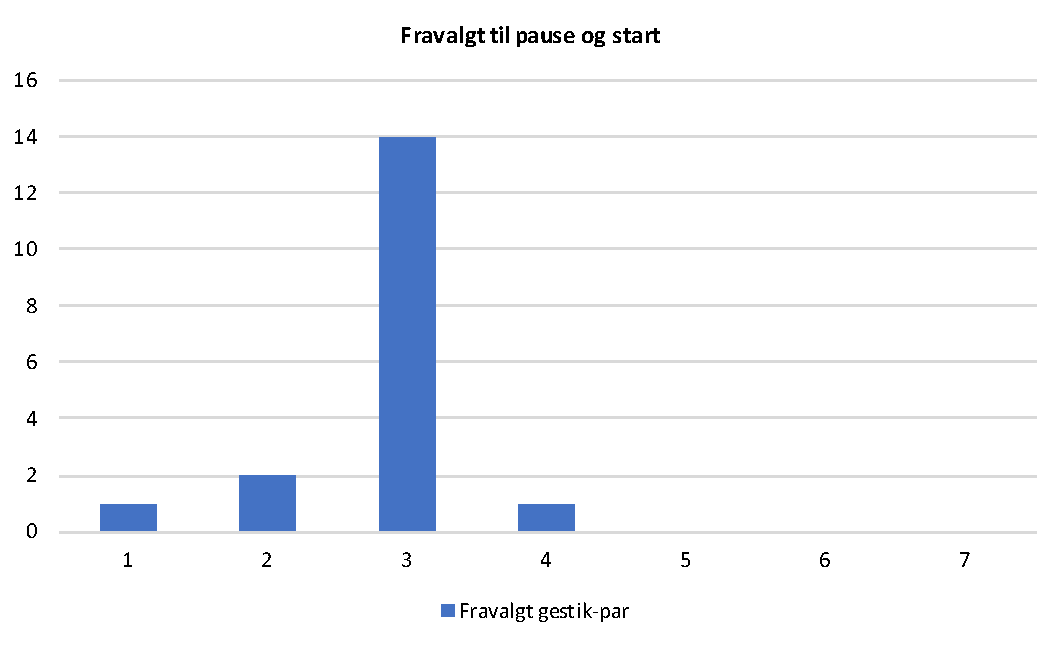
\includegraphics[resolution=300,width=0.9\textwidth]{Test1/DatabehandlingGrafer/FravalgtPause}
	\caption{Barplot over hvilke gestik-par testpersonerne fravælger i forbindelse med pause og start.}
	\label{fig:DaarligstGestikPause}
\end{figure}
\noindent
% 
På \autoref{fig:DaarligstGestikPause} fremgår det hvilke gestik-par de 18 testpersoner fravælger i forbindelse med at skulle pause og starte musikken. Det fremgår tydeligt at gestik-par 3 er det par, som flest testpersoner fravælger i forhold til de tre andre gestik-par, der ellers er repræsenteret på \autoref{fig:DaarligstGestikPause}. Derudover fravælges gestik-par 1 af én testperson, testperson 13, fordi testpersonen forbinder det med at række en hånd i vejret. Testperson 1 og testperson 8 fravælger gestik-par 2 på baggrund af bevægelsesmængden, hvor begge testpersoner giver udtryk for, at der er for meget unødvendig bevægelse. Årsagen til at testperson 5 fravælger gestik-par 4 skyldes at testpersonen generelt ikke bryder sig om at pege. I og med at testperson 5 både kommenterer at den er lidt aggressiv og at det vil føles lidt mærkeligt at stå derhjemme og pege, så tyder det på at testpersonen oplever gestik-par 4 som værende social uacceptabel. 

De resterende 14 testpersoner fravælger alle gestik-par 3. De to største årsager til at parret fravælges er på grund af kompleksiteten i bevægelsen og at det simpelthen er for besværeligt at udføre. I forhold til bevægelsen giver flere testpersoner udtryk for at den, foruden at være kompleks, enten er for underlig, testperson 3, for mærkelig, testperson 4, for lang og akavet, testperson 7 og for indviklet, testperson 12. I tillæg kommenterer testperson 17, at det bliver en større øvelse at skulle pause og starte musikken, og så vil der gå lang tid før musikken rent faktisk bliver sat på pause. Derudover giver testperson 14 og testperson 15 udtryk for, at det ikke er sikkert, at de kan huske hvordan bevægelsen er, når den så skal udføres. I tillæg kommenterer testperson 14 at hun simpelthen ikke ville vide, hvordan hun skulle tænde eller slukke for lyden, svarende til at sætte musikken på pause og starte den igen. Testperson 9 giver udtryk for lignede bekymringer omkring hvordan musikken sættes på pause og startes igen.

Af de 18 testpersoner, der har deltaget i testen, er der kun to, testperson 8 og testperson 13, som har inkluderet gestik-par 3 i deres rangering. Begge testpersoner vælger gestik-par 3 som deres første prioritet, lige indtil at testperson 8 til sidst skal gengive de fortrukne gestikker og indtil testperson 13 skal lave en forbedring, hvorefter gestik-parret, i begge tilfælde, rangeres som den næstbedste. Årsagerne til at testperson 8 har inkluderet gestik-par 3 blandt de tre bedste er dels at den er unik, speciel og sjov, men den gav også en fornemmelse af at det ikke bare var en knap der blev trykket på. Testperson 13 inkluderer derimod gestik-par 3 fordi det ikke er typisk ting at gøre og dermed ikke vil komme til at pause musikken ved et uheld.\blankline
%
For at afgøre hvilke af de syv gestik-par, der skal fravælges, er det nødvendigt at sammenholde hvilke gestikker testpersonerne fravælger med de gestikker, som indgår i testpersonernes top tre rangering. Der opstilles derfor en tabel over de fire fravalgte gestik-par og hvordan de indgår i testpersonernes rangering.
%
\begin{table}[H]
	\centering
	\begin{tabular}{ | p{2.4cm} | p{2.4cm} | p{2.4cm} | p{2.4cm} | p{2.4cm} |}
	\hline
		 & Gestik-par 1 & Gestik-par 2 & Gestik-par 3 & Gestik-par 4 \\ \hline
		1. Plads & 8 & 1 & 0 & 0\\ \hline
		2. Plads & 3 & 3 & 2 & 1\\ \hline
		3. Plads & 2 & 0 & 0 & 2\\ \hline
	\end{tabular}
	\caption{Oversigt over hvor ofte og hvor de fire fravalgte gestikker indgår i testpersonernes top tre rangering.}
	\label{tab:FravalgteTopTrePause}
\end{table}
\noindent
%
På baggrund af \autoref{tab:FravalgteTopTrePause} tyder det på, at det eneste gestik-par, der flerstemmigt kan ekskluderes, er gestik-par 3, dels fordi parret kun indgår i to testpersoners top tre og dels fordi 14 testpersoner har fravalgt det. Derudover er gestik-par 4 kun inkluderet tre gange i testpersonernes samlede top tre rangering, jævnfør \autoref{tab:FravalgteTopTrePause}, og da gestik-parret ydermere er fravalgt, blandt andet på baggrund af det er socialt uacceptabelt, besluttes det at dette par ligeledes ekskluderes fra fremtidige undersøgelser. 

I forhold til gestik-par 2 så tyder det på, at parret kun indgår i testperson 3's rangering, fordi testpersonen forbinder de andre forslag med mute og testpersonen giver derefter udtryk for, at det ikke giver meningen at lave et dynamisk stop-tegn, svarende til gestik-par 2. Der skal dog tages forbehold for at testperson 3, ud fra testpersonens respons, virker forvirret og selvmosigende. Ifølge testperson 7 bliver gestik-par 2 inkluderet i top tre, fordi den virkede lige til og at det er det testpersonen forstår ved et stop-tegn. Årsagen til at testperson 10 inkluderer gestik-par 2 kan ikke direkte udledes af det indsamlede data, men generelt har testpersonen valgt gestikker, som var nemme at huske og med en lille risiko for at gestikken enten gengives forkert ved en forkert bevægelse eller udføres ved et uheld. Den eneste testperson, som har gestik-par 2 på en første plads i sin top tre er testperson 12 og årsagen til det er fordi testpersonen som udgangspunkt ville have valgt gestik-par 1, som den bedste og forbedret parret ved at tilføje bevægelsen, der allerede er inkluderet i gestik-par 2. Men derudover nævner testperson 12 også at være fascineret af gestik-par 5, hvorfor det vurderes at det måske også vil tilfredsstille testpersonen, hvis gestik-par 5 blev valgt. 

Argumenterne for at fravælge gestik-par 2 kan, blandt andet, sammenholdes med responsen fra både testperson 1 og testperson 8, som begge vurderer, at der er unødvendigt meget bevægelse i. Derudover blev i \fullref{Socialaccept}, blandt andet, inddraget en undersøgelse hvori det blev konkluderet at testpersonerne følte sig mest komfortable når afstanden mellem dem og selve interaktionen var lille, hviket ligeledes understøtter argumenterne for at fravælge gestik-par 2. Selvom fokus for denne del af undersøgelsen ikke vedrører social accept, så tyder det på, at desto tættere på kroppen gestikkerne udføres, desto større er sandsynligheden for at de indgår på testpersonernes top tre. Så baseret på de foregående argumenter og fordi gestik-par 2 kræver en bevægelse langt fra kroppen, i forhold til de andre forslag samt at gestik-parret kun fremgår fire gange i testpersonernes top tre, jævnfør \autoref{tab:FravalgteTopTrePause}, så vælges det at ekskludere gestik-par 2 fra fremtidige undersøgelser. 
%
\section{Fravælgelse af gestik-par til at skifte musiknummer}
\label{app:TestresultaterSkiftDaarlig}
%
I følgende afsnit analyseres hvilke af de syv semaforiske gestik-par testpersonerne fravælger samt hvorfor testpersonerne netop fravælger disse gestik-par. På baggrund af analysen bør det være muligt at udpege hvilke semaforiske gestikker, der i hvert fald ikke skal knyttes til at skifte musiknummer. Analysen bygger på testpersonerne respons til spørgsmålet: \textit{Hvilken gestik kan du mindst lide? og hvorfor?}, hvor testpersonernes samlede data er vedlagt i ELEKTRONISK BILAG.
%
\begin{figure}[H]
	\centering
	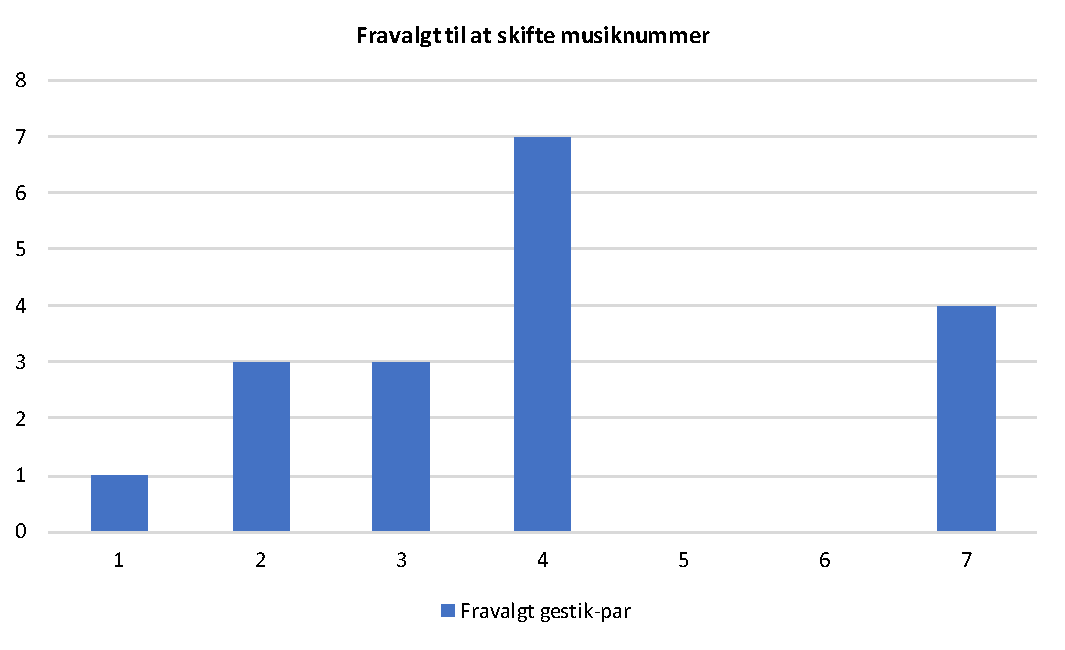
\includegraphics[resolution=300,width=0.9\textwidth]{Test1/DatabehandlingGrafer/FravalgtSkift}
	\caption{Barplot over hvilke gestik-par testpersonerne fravælger i forbindelse med at skifte musiknummer frem og tilbage.}
	\label{fig:DaarligstGestikSkift}
\end{figure}
\noindent
%
På \autoref{fig:DaarligstGestikSkift} fremgår det, hvilke gestik-par de 18 testpersoner fravælger i forbindelse med at skifte musiknummer. Det fremgår tydeligt at gestik-par 4 er det gestik-par, som flest testpersoner fravælger i forhold til de resterende par på \autoref{fig:DaarligstGestikSkift}. Derudover fravælges gestik-par 7 næstflest gange, mens gestik-par 2 og gestik-par 3 frevælges 3 gange og gestik-par 1 fravælges en enkelt gang. Årsagen til at testperson 14 har valgt gestik-par 1, som værende den testpersonen mindst kan lide, begrundes med at testpersonen forestiller sig, at det er en bevægelse testpersonen vil komme til at gøre gentagende gange foran sit anlæg eller under en samtale. Testperson 1, testperson 5 og testperson 16 har alle valgt gestik-par 2, som værende den de mindst kan lide, fordi gestikken er modsat af, hvad de forventer er frem og tilbage. At gestik-par 3 fravælges begrunder testperson 3, testperson 11 og testperson 13 med, at hvis der skulle peges i en retning så skulle det være med pegefingeren og ikke tommelfingeren, da det er en akavet bevægelse og fordi gestikken er statisk. I den forbindelse kommenterer testperson 5 at vedkommende heller ikke bryder sig om hverken gestik-par 3 eller gestik-par 7, netop fordi de er statiske.

Der er forskellige årsager til at syv testpersoner fravælger gestik-par 4. Testperson 4 og testperson 6 fravælger gestikken, fordi den er mærkelig, hvor testperson 4 forbinder det med at skulle tage telefonen. Testperson 8 forstår ikke, hvorfor det er lige præcis er det håndtegn, der skal bruges. Testperson 10 oplever ikke at gestikken bringer noget nyt, men snarere at det er en besværlig version af gestik-par 5. I forhold til håndtegnet i gestik-par 4, så kommenterer testperson 12 at det er unaturligt at gøre noget med lillefingere, testperson 7 kommenterer dels, at det er en stor armbevægelse og dels, at det er et sjovt håndtegn, som vil blive glemt, hvis det ikke bliver brugt. I tillæg kommenterer testperson 18 ligeledes at det er en unaturlig gestik, som vil blive glemt. Dog pointerer testpersonen at det er en effektiv gestik i og med at den ikke vil blive lavet ved en fejl. 

Årsagen til at gestik-par 7 fravælges skyldes ifølge testperson 2, testperson 9 og testperson 17, dels at den virkede mærkelig, dels at den ikke blev opfattet og dels at den minder lidt om en pistol. Ligesom gestik-par 3 blandt andet blev fravalgt, fordi den er statisk, så fravælger testperson 15 af samme årsag gestik-par 7 samt at det er et enkelt tegn.\blankline
%
For at afgøre hvilke af de syv gestik-par, der skal fravælges, er det nødvendigt at sammenholde hvilke gestikker testpersonerne fravælger med de gestikker, som indgår i testpersonernes top tre rangering. Der opstilles derfor en tabel over de fem fravalgte gestik-par og hvordan de indgår i testpersonernes rangering.    
%
\begin{table}[H]
	\centering
	\begin{tabular}{ | p{1.5cm} | p{2.1cm} | p{2.1cm} | p{2.1cm} | p{2.1cm} | p{2.1cm} |}
	\hline
		 & Gestik-par 1 & Gestik-par 2 & Gestik-par 3 & Gestik-par 4 & Gestik-par 7 \\ \hline
		1. Plads & 10 & 3 & 1 & 0 & 0\\ \hline
		2. Plads & 2 & 3 & 3 & 0 & 1\\ \hline
		3. Plads & 0 & 0 & 7 & 5 & 2\\ \hline
	\end{tabular}
	\caption{Oversigt over hvor ofte og hvor de fem fravalgte gestikker indgår i testpersonernes top tre rangering.}
	\label{tab:FravalgteTopTreSkift}
\end{table}
\noindent
%
På baggrund af \autoref{tab:FravalgteTopTreSkift} sammenholdt med \autoref{fig:DaarligstGestikSkift}, tyder det på at gestik-par 4 og gestik-par 7 kan ekskluderes fra fremtidige undersøgelser. Det skyldes at selvom gestik-par 4 indgår fem gange i testpersonernes top tre, så fravælges parret af syv testpersoner. Derudover tyder det på, at de fem testpersoner, som har inkluderet gestik-par 4 i deres top tre, har gjort det på baggrund af bevægelsen snarre end kombinationen af både håndtegnet og bevægelsen. Gestik-par 7 ekskluderes, da parret kun indgår tre gange i top tre og da den derudover fravælges af fire testpersoner. 

De tre testpersoner, som fravælger gestik-par 2, gør det formentligt fordi de har en mental model af, at hvis der swipes fra højre mod venstre så afspilles det næste musiknummer i playlisten, modsat hvis der swipes fra venstre mod højre så afspilles det forrige musiknummer. De tre testpersoner, der har inkluderet gestik-par 2 som deres første valg, har formentligt den modsatte mentale model af hvilken swipe bevægelse der skal udføres for at skifte til det næste musiknummer. For at det kan afgøres hvorvidt gestik-par 2 skal ekskluderes eller ej, så er det nødvendigt at undersøge nærmere hvilke gestik-par de seks testpersoner, som har inkluderet gestik-par 2 i deres top tre, ellers har inkluderet. 
%
\begin{table}[H]
	\centering
	\begin{tabular}{ | p{3cm} | p{3cm} | p{3cm} | p{3cm} |}
	\hline
		 & 1. Plads & 2. Plads & 3. Plads \\ \hline
		Testperson 4 & Gestik-par 2 & Gestik-par 5 & Gestik-par 3 \\ \hline
		Testperson 17 & Gestik-par 2 & Gestik-par 3 & Gestik-par 4 \\ \hline
		Testperson 18 & Gestik-par 2 & Gestik-par 1 & Gestik-par 3 \\ \hline
		Testperson 8 & Gestik-par 3 & Gestik-par 2 & Gestik-par 7 \\ \hline
		Testperson 12 & Gestik-par 1 & Gestik-par 2 & Gestik-par 5\\ \hline
		Testperson 15 & Gestik-par 1 & Gestik-par 2 & Gestik-par 5 \\ \hline
	\end{tabular}
	\caption{Oversigt over de seks testpersoner, som enten har tildelt gestik-par 2 en første eller en anden plads i top tre, samt hvilke gestik-par de ellers har inkluderet.}
	\label{tab:GestikPar2ITopTre}
\end{table}
\noindent
%
Sammenholdes testperson 4's top tre rangering med testpersonens udsagn og bevægelser i videooptagelserne, så tyder det på at denne testperson har en mental model af, at hvis der swipes fra højre mod venstre så afspilles det forrige musiknummer kontra et swipe fra venstre mod højre, som vil afspille det næste musiknummer. Testpersonen kommenterer ydermere at gestik-par 5 også vil fungere såfremt retning var omvendt, svarende til hvad der sker i gestik-par 2. Testperson 17, som også har rangeret gestik-par 2 som det bedste, udfører også de korrekte bevægelser i forhold til testpersonens egne kommenterer, dog opstår der en smule usikkerhed, når testpersonen afslutningsvist skal gengive sine fortrukne gestikker. Efter en diskusion frem og tilbage med testlederen konkluderer testperson 17 dog at det stadig er gestik-par 2, der er bedst. Selvom testperson 18 virker sikker i sit valg om, at det er gestik-par 2, der er det bedste gestik-par, så gengiver testpersonen rent faktisk bevægelserne fra gestik-par 1, dog med venstre hånd. Når testpersonen i tillæg forklarer hvad swipe bevægelserne gør i forhold til at skifte til det forrige eller det næste musiknummer, relaterer det sig ligeledes til gestik-par 1. Det er derfor ikke til at vide hvorfor testpersonen har rangeret gestik-par 2 højere end gestik-par 1. Det tyder derfor på at den eneste testperson, der med sikkerhed vil vælge swipe bevægelserne i gestik-par 2, er testperson 4. 

Rettes fokus mod de tre testpersoner, som har rangeret gestik-par 2 på en anden plads, så tyder det på at de to testpersoner, som har gestik-par 1 på en første plads, hovedsageligt har inkluderet gestik-par 2 på grund af bevægelsen. Dog kommenterer testperson 15, at gestik-par 2 er modsat af hvad testpersonen finder logisk, i forhold til at skifte musiknummer.  Derudover pointerer testperson 12, at det var svært at adskille gestik-par 1 fra gestik-par 2. Testperson 8 har derimod rangeret gestik-par 2 mellem de to statiske gestik-par og når testpersonen gengiver bevægelserne for gestik-par 2 så stemmer det både overens med testpersons udsagn samt hvordan gestik-parret er designet. Det tyder derfor på at testpersonen rent faktisk har valgt gestik-par 2 fordi det stemmer overens med testpersonens mentale model.\blankline 
%
Ud af de seks testpersoner er det kun testperson 4 og testperson 8, der rent faktisk giver entydigt udtryk for at deres mentale model af gestik-par 2 stemmer overens både med deres bevægelser og deres udsagn. Derudover er der i Bang $\&$ Olufsen's produkter desuden truffet en designbeslutning om, at en swipe bevægelse fra højre mod venstre resulterer i at det er det næste musiknummer afspilles, da dette stemmer overens med at trække der næste musiknummer frem. På baggrund af den foregående analyse og da det ikke ønskes at gå i mod Bang $\&$ Olufsen's designvalg, vurderes det derfor at der er tilstrækkeligt belæg for at ekskludere gestik-par 2. 

På baggrund af foregående analyse forefindes der ikke et tilstrækkeligt belæg for hverken at ekskludere gestik-par 1 eller gestik-par 3, hvorfor disse vil undersøges nærmere. 
%
\section{Fravælgelse af gestik-par til at skrue op og ned for musikken}
\label{app:TestresultaterVolumenDaarlig}
%
I følgende afsnit analyseres hvilke af de ni semaforiske gestik-par testpersonerne fravælger samt hvorfor testpersonerne netop fravælger disse gestik-par. På baggrund af analysen bør det være muligt at udpege hvilke semaforiske gestikker, der i hvert fald ikke skal knyttes til at skrue op og ned for musikken. Analysen bygger på testpersonerne respons til spørgsmålet: \textit{Hvilken gestik kan du mindst lide? og hvorfor?}, hvor testpersonernes samlede data er vedlagt i ELEKTRONISK BILAG.
%
\begin{figure}[H]
	\centering
	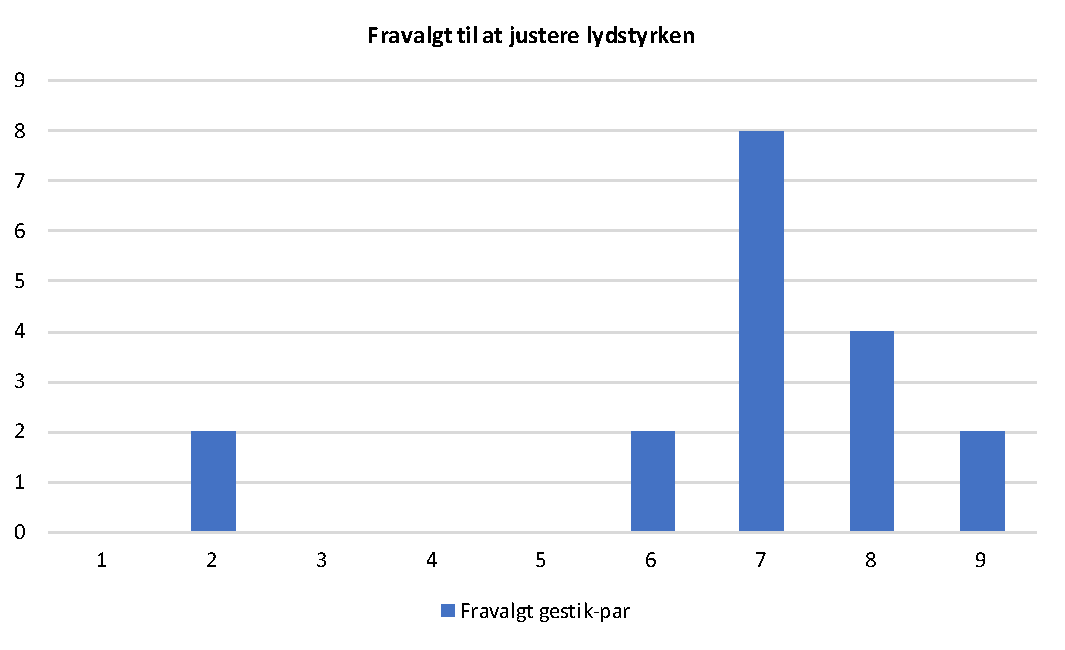
\includegraphics[resolution=300,width=0.9\textwidth]{Test1/DatabehandlingGrafer/FravalgtVolumen}
	\caption{Barplot over hvilke gestik-par testpersonerne fravælger i forbindelse med at skrue op og ned for musikken.}
	\label{fig:DaarligstGestikVolumen}
\end{figure}
\noindent
%
På \autoref{fig:DaarligstGestikVolumen} fremgår det, hvilke gestik-par de 18 testpersoner fravælger i forbindelse med at skrue op og ned for musikken. Det fremgår tydeligt at testpersonerne hyppigst fravælger gestik-par 7, da gestik-parret i alt er fravalgt otte gange, og ikke indgår på en eneste top tre rangering, hvilket fremgår af \autoref{tab:GestikParITopTreVolumen}. Årsagen til at gestik-par 7 fravælges varierer mellem de otte testpersonerne, som har valgt parret. Testperson 2 har svært ved at vurdere hvilken vej der er op og hvilken vej der er ned. Ifølge testperson 3 er gestik-par 7 underligt og derudover så giver den ikke mening. At gestik-parret ikke giver mening pointere testperson 15 også og tilføjer, at det er en mellemting mellem gestik-par 5 og gestik-par 6. Testperson 4 fravælger gestikken, fordi den er mærkelig, hvilket også er en af årsagerne til at testperson 11 fravælger parret. Derudover kommenterer testperson 11, at det kræver koncentration at lave en bue, hvilket er en del af bevægelsen. Da formålet med at anvende semaforiske gestikker til at interagere med Bang $\&$ Olufsen's fremtidige musikanlæg, blandt andet er for at interaktionen på sigt kan foregå i den perifere opmærksomhed, så er det ikke hensigtsmæssigt at gestikkerne kræver mere koncentration end andre løsninger. Derudover påpeger testperson 10 at gestik-par 7 er væsentligt mindre intuitiv end de andre forslag og dertil er det svært at vurdere den nødvendige bevægelsesmængde for at skrue op og ned. Ifølge testperson 6 så er gestik-par 7 det par, som skiller sig mest ud i forhold til de andre forslag, hvilket er årsagen til at parret fravælges. Testperson 14's respons afviger fra de andre testpersoners, i det at testperson 14 fravælger gestik-par 7, fordi testpersonen anser det som værende en meget naturlig bevægelse, som testpersonen giver udtryk for at ville komme til at lave ubevidst.

Selvom gestik-par 7 blev inkluderet som et forsøg på at overfører gestikken, der anvendes til at skrue op og ned på en A9, \parencite{WEB:BeoplayA9}, til en semaforisk gestik, så er gestik-par 7 det par, som oftes fravælges og som ikke indgår i nogen af testpersonernes top tre, hvorfor parret ekskluderes.\blankline
%
To ud af de fire testpersoner, som fravælger gestik-par 8, giver udtryk for at det er besværligt at pege nedad. Den ene af de to, testperson 18, giver stærkt udtryk for at det er både besværligt og ubehagligt at pege nedad samt at have sin arm i den position. Den anden af de to testpersoner, testperson 9, giver udtryk for at det besværligt at bruge og det er underligt at pege nedad. Derudover pointere testperson 9 at det er svært at kontrollere, hvor meget der enten skal skrues og eller ned, hvilket også er årsagen til at testperson 5 fravælger gestik-par 8; der er ingen mulighed for at kontrollere hvor meget der skrues op. Den sidste af de fire testpersoner, testperson 13, fravælger gestik-par 8 fordi der mangler bevægelse og fordi det er noget testpersonen godt kunne forestille sig komme til at gøre ved et uheld. \blankline 

Der er to forskellige årsager til hvorfor gestik-par 2 fravælges af testperson 12 og testperson 16. Testperson 12 fravælger gestik-par 2, fordi testpersonen ikke bryder sig om cirkelbevægelsen, selvom testpersonen pointere at det burde virke naturligt og det egentlig er sådan der normaltvist skrues op på et anlæg. Det skal dog pointeres at testperson 12 ikke endegyldigt fastslår at det er gestik-par 2, der er værst, da testpersonen egentlig heller ikke bryder sig om gestik-par 1. Grunden til at det fremgår, at testperson 12 har valgt gestik-par 2 som værende dårligst, er på baggrund af de bevægelser, der opstår når testpersonen skal forklare hvorfor der vælges som der gør. I dette tilfælde stemte bevægelsen overens med bevægelsen i gestik-par 2. Årsagen til at gestik-par 2 fravælges af testperson 16, er fordi bevægelsen er modsat af hvad testpersonen ville forvente. Det skal dog pointeres at der ved gestik-par 2 skrues op for musikken ved at dreje hånden med uret og skrues ned ved at dreje hånden mod uret, hvilket er det testpersonen egentlig forventer. Det tyder derfor på at testperson 16 har misforstået videooptagelsen af gestik-par 2. Testlederen spørger derfor ind til hvordan gestik-par 2 kunne gøres bedre, hvor testperson 16 først og fremmest foreslår at bevægelsen foregår i den rigtige retning og derudover foreslår testpersonen at gestikken skulle være mere ligesom gestik-par 1, hvor testpersonen referer til armens position. 

Gestik-par 6 fravælges af testperson 9 fordi det vil være svært at gengive bevægelsen med et barn på armen, hvilket også gør sig gældende for gestik-par 5. Testperson 17 fravælger gestik-par 6 fordi det er ulogisk at lave den bevægelse i forbindelse med musik og derudover virker det mærkelig at begge hænder skal være involveret. 

Ifølge testperson 7 så fravælges gestik-par 9 fordi den ikke tillader kontrol over hvor meget der skrues op og ned, hvorimod testperson 8 fravælger gestik-par 9 fordi testpersonen vil have det akavet med at lave den bevægelse.\blankline
%
For at afgøre hvilke af de ni gestik-par, foruden gestik-par 7, som allerede er ekskluderet, der skal fravælges, er det nødvendigt at sammenholde hvilke gestikker testpersonerne fravælger med de gestikker, som indgår i testpersonernes top tre rangering. Der opstilles derfor en tabel over de fem fravalgte gestik-par og hvordan de indgår i testpersonernes rangering.    
%
\begin{table}[H]
	\centering
	\begin{tabular}{ | p{1.5cm} | p{2.1cm} | p{2.1cm} | p{2.1cm} | p{2.1cm} | p{2.1cm} |}
	\hline
		 & Gestik-par 2 & Gestik-par 6 & Gestik-par 7 & Gestik-par 8 & Gestik-par 9 \\ \hline
		1. Plads & 4 & 1 & 0 & 0 & 2\\ \hline
		2. Plads & 2 & 2 & 0 & 0 & 1\\ \hline
		3. Plads & 3 & 1 & 0 & 2 & 3\\ \hline
	\end{tabular}
	\caption{Oversigt over hvor ofte og hvor de fem fravalgte gestikker indgår i testpersonernes top tre rangering.}
	\label{tab:FravalgteTopTreVolumen}
\end{table}
\noindent
%
På baggrund af \autoref{tab:FravalgteTopTreVolumen} hvor gestik-par 9 fremgår seks gange i testpersonernes top tre rangering sammenholdt med \autoref{fig:DaarligstGestikVolumen} samt testpersonernes begrundelser for hvorfor de fravælger gestik-par 9, vurderes det at der er ikke er belæg for at ekskludere gestik-par 9. Det vurderes ydermere at der ikke forefindes tilstrækkeligt belæg for at ekskludere gestik-par 2, for selvom det ikke kan antages med sikkerhed, at testperson 16 ville have udpeget et andet gestik-par, i tilfælde af at testpersonen ikke havde misforstået bevægelsesretningen, så tyder det på, at det godt kunne være tilfældet. I så fald er det kun testperson 12, som har givet udtryk for at en cirkulærbevægelse ikke foretrækkes. Da det heller ikke entydigt kan konkluderes, hvorvidt testperson 12 mindst kan lide gestik-par 2 i forhold til gestik-par 1 og da gestik-par 2 sammenlagt indgår ni gange i testpersonernes top tre, jævnfør \autoref{tab:FravalgteTopTreVolumen}, vurderes det at der ikke er belæg for at ekskludere gestik-par 2 .\blankline 
%
Baseret på \autoref{tab:FravalgteTopTreVolumen} hvor gestik-par 8 kun indgår to gange i testpersonernes samlede top tre rangering sammenholdt med \autoref{fig:DaarligstGestikVolumen} samt testpersonernes begrundelser for, hvorfor de fravælger gestik-par 8, vurderes det at der er belæg for at ekskludere gestik-par 8.  

For at have belæg for at ekskludere gestik-par 6 er det nødvendigt at inkludere hvad testpersonerne, som har rangeret gestik-par 6 i deres top tre, har kommenteret. Ifølge testperson 1 så indgår gestik-par 6 på en anden plads dels fordi den følger et princip om noget, der er større eller mindre og dels fordi bevægelsen er naturlig. Det tyder på at testperson 14 rangerer gestikker alt efter hvad der føles akavede og unaturligt i frygt for at komme til at lave gestikkerne ved et uheld, hvilket er årsagen til at testperson 14 har tildelt gestik-par 6 en anden plads. Testperson 2 forklarer at årsagen til at gestik-par 6 rangeres på en tredje plads, er fordi den minder om gestik-par 4 og gestik-par 5 bare sidelæns, men at det ikke giver lige så meget mening, som de to andre. Baseret på testperson 5's udsagn tyder det på at årsagen til at gestik-par 6 tildeles en første plads er fordi testpersonen ønsker at have fuld kontrol over, hvor meget der skrues op og ned, hvilket testpersonen oplever ved at bruge begge hænder. Grunden til at testpersonen vælger gestik-par 6 fremfor gestik-par 5 skyldes, at testpersonen derved føler sig mindre i rummet. Sammenholdes de fire testpersoners udsagn med hvordan de rent faktisk gengiver gestik-par 6, så tyder det på, at ingen af testpersonerne formår, at gengive bevægelsen korrekt. Det fremgår af optagelserne at ingen af de fire testpersoner formår at fastholde deres ikke-dominante hånd, som reference og derfra kontrollere hvor meget der skal skrues op eller ned med den dominante hånd. Til gengæld tyder det på at de fire testpersoner fortolker og gengiver gestik-par 6 ens; begge hænder bevæger sig horisontalt mod eller væk fra hinanden med håndfladerne vendt ind mod hinanden. 

Så med udgangspunkt i testpersonerne begrundelser for hvorfor de enten fravælger gestik-par 6 eller inkluderer gestik-par 6 i deres top tre, samt hvad de rent faktisk gør, når de gengiver gestik-parret, så vurderes det at der er belæg for at ekskludere gestik-par 6.  






\chapter{Instruktioner til værten}
\label{app:InstruktionerVaert}
%
De følgende instruktioner er anvendt af testleder 1, som har ansvaret for familiarisering af testpersonen, der agerer gæst. \blankline
%
\textit{Først vil jeg gerne bede dig om at læse og underskrive denne samtykkeerklæring. Sig endelig til, hvis du har nogle spørgsmål.}\blankline
%
Testlederen udlevere samtykkeerklæringen til testpersonen, som læser og underskriver den. \blankline
%
\textit{Du har fået et nyt musikanlæg, som kan styres ved brug af semaforiske gestikker; håndbevægelser. Du skal sammen med mig lære at styre dit musikanlæg med de her gestikker. Først får du vist gestikkerne på en film, hvorefter vi gennemgår dem og du får lov at prøve dem til musik. Til sidst får du lov at styre musikken ved hjælp af forskellige hints, og når du kan finde ud af det, forlader jeg lokalet, hvorefter du skal øve dig i at styre musikken til de her hints. Når du har lært at styre musikanlægget får du besøg af din ven(inde)/kæreste og I skal sammen planlægge en ferie på to uger. Under planlægningen af ferien vil I høre musik, og vi vil præsentere de forskellige hints, som du skal reagere på, på den måde vi har øvet.}\blankline
%
Testlederen og værten ser videoen.\blankline
%
\textit{Nu kan du så prøve at styre selve musikanlægget. Når du laver gestikkerne må du gerne rette dem hen imod anlægget.}\blankline
%
Værten prøver at styre musikanlægget uden hints og derefter med hints. \blankline
%
\textit{Når telefonen ringer, må du gerne tage den og holde den op til øret. Derudover er det vigtigt du kun reagerer på de forskellige hints, når du prøver alene her i lokalet og når du får besøg.}\blankline
%
Testlederen forlader lokalet og værten styrer musikken ved hjælp af de forskellige hints. Efter værten har gennemgået familiariseringen kommer gæsten ind. \blankline
%
\textit{Nu skal I så planlægge en ferie sammen. I har alle hjælpemidler til rådighed, så I slår jer bare løs. Imens I planlægger ferie vil I høre musik, hvor værten lige kan starte med at justere lydstyrken, så I kan snakke sammen. Ellers god fornøjelse med planlægningen!}\blankline
%
Værten og gæsten planlægger ferie, mens værten interagerer med musikanlægget, når de forskellige hints bliver præsenteret.\blankline
%
\textit{Hej igen! Jeg håber I har fået planlagt noget godt, for nu får I ikke mere tid her. Jeg vil gerne bede gæsten om at gå ud og snakke lidt med testleder 2, så snakker jeg lidt med værten.}

\chapter{Instruktioner til gæsten}
\label{app:InstruktionerGaest}
%
De følgende instruktioner er anvendt af testlederen, som instruerer testpersonen, som agerer gæst, i hvad gæstens opgave er.\blankline
%
\textit{Din opgave er at planlægge tre forskellige ferier, som dig og din ven(inde)/kæreste skal på. Den ene ferie er en budget ferie hvor I har 10000kr. til rådighed, en standard ferie hvor I har 20000kr. til rådighed og en luksus ferien hvor I har +30000kr. til rådighed. De tre ferier skal vare to uger, og hvor I skal hen det er op til dig men du skal også finde ud af hvordan I kommer derhen, hvor I skal overnatte og hvad I skal opleve og samtidig have et madbudget. Så med andre ord så er det alt der skal planlægges. Du har de her fem hjemmesider til rådighed, der er; momondo, trivago, hotels.com, tripadvisor og airbnb, hvis du kender andre hjemmesider, som du hellere vil bruge så må du selvfølgelig også det. Vi regner ikke med at du når, at planlægge det hele her ude og det er heller ikke meningen, for når de er færdige derinde, så skal du på besøg hos din ven(inde)/kæreste og så skal I sammen planlægge videre på de tre ferier. Når du så kommer på besøg hos din ven(inde)/kæreste så skal du præsentere dine ferieforslag og skal I sammen planlægge videre på dem.}\blankline
%
\textit{Da vi gerne vil have lov til at optage Jer derinde, så vil jeg bede dig om at læse den her samtykkeerklæring og hvis du har nogle spørgsmål, så sig endelig til.}\blankline
%
Testpersonen læser og underskriver samtykkeerklæringen.\blankline
%
\textit{Når de er færdige derinde så bliver du hentet. På det her papir er opgaven opsummeret så du kan se hvad du skal huske at tage højde for i din ferieplanlægning.}\blankline
%
Testlederen lægger papiret frem hvor opgaven er opsummeret. \blankline
%
\textit{Du får den her blok papir og en kuglepen, som du kan bruge til at skrive nogle af dine idéer ned på.}\blankline
%
\textit{Når du kommer på besøg hos din ven(inde)/kæreste så har han/hun fået et nyt musikanlæg, som i kommer til at høre musik fra imens I planlægger ferien. Din ven(inde)/kæreste vil komme til at styre det undervejs, men det behøver du ikke at tænke over, fordi din opgave er at få præsenteret dine ferieforslag og planlæg videre med din ven(inde)/kæreste. Har du nogle spørgsmål?}




\chapter{Opgaver til gæsten}
\label{app:OpgaverTilGaesten}
%
Du skal starte planlægnigen af:\blankline
\begin{enumerate}
	\item En budgetferie til omkring 10.000 kr for dig og din ven(inde)/kæreste
	\item En standard ferie til omkring 20.000 kr for dig og din ven(inde)/kæreste
	\item En luksusferie til +30.000 kr for dig og din ven(inde)/kæreste\blankline
\end{enumerate}
%
Priserne skal dække:\blankline
\begin{itemize}
	\item Hvordan I kommer derhen
	\item Hvor I skal overnatte
	\item Hvad I skal opleve
	\item Madbugdet
\end{itemize}
\Chapter{Cheat sheet til værten}
\label{app:CheatSheetTilVaerten}





\end{document}
 